\chapter{Взаимодействие экстремально интенсивного лазерного излучения с твердотельной мишенью}\label{ch:ch2}

\section{Введение}\label{sec:ch2/sec1}
В предыдущей главе было показано, что реакция излучения может существенно влиять на динамику частиц в сильных ЭМ полях.
Помимо реакции излучения, существует еще один важный эффект, который оказывает значительное влияние на поведение вещества в экстремальных ЭМ полях~---~развитие КЭД \textit{каскадов}~\cite{sturrock1971model,daugherty1982electromagnetic,nerush2007radiation,Bell2008,Nerush11a,Ridgers12,narozhny2015quantum,Kostyukov2016,nerush2017weibel,efimenko2019laser,yakimenko2019prospect}.
Они возникают в результате излучения жестких фотонов ультрарелятивистскими частицами, и последующего распада первых на электрон-позитронные пары в результате нелинейного процесса Брейта-Уилера или нелинейного трайдент процесса.
Вторичные частицы также вовлекаются в излучение фотонов и фоторождение пар, что приводит к лавинообразному росту количества частиц.
Одной из главных причин того, что развитие КЭД каскадов пока ещё не было продемонстрировано экспериментально, состоит в том, что данный феномен является пороговым по интенсивности ЭМ поля.
Это в свою очередь связано с экспоненциально малой вероятностью процесса Брейта-Уилера и трайдент процесса в области параметров $\chi\lesssim 1$, где $\chi$~---~КЭД параметр фотонов, определяемый следующим образом
\begin{equation}
    \chi = \frac{\varepsilon}{a_\mathrm{S}} \sqrt{{\left( \vb{E} + \vb{v}\times\vb{B} \right)}^2 - {\left(\vb{v}\vb{E} \right)}^2} ,
\end{equation}
где $\varepsilon$ и $\vb{v}\equiv\vb{k}/k$~---~энергия, нормированная на $mc^2$, и направление распространения фотона соответственно, $\vb{k}$~---~волновой вектор фотона.
Для оценки параметров лазерного излучения, требуемых для наблюдения КЭД каскада, обычно предполагают, что характерная энергия электрона в поле лазера равна по порядку величины $a_0$.
Таким образом, условие $\chi>1$, требуемое для развития КЭД каскада, записывается через интенсивность излучения как $I[\SI{e23}{\watt/\centi\meter^2}]\lambda[\si{\um}]\gtrsim 5$.
Данная оценка кажется довольно оптимистичной применительно к упомянутым во введении лазерным установкам нового поколения, работающим в оптическом диапазоне $\lambda\approx\SI{1}{\um}$, и на которых ожидаются интенсивности порядка ${I\sim\SI{e24}{\watt/\centi\meter^2}}$.
Однако, из-за порогового характера КЭД каскада, представленная выше грубая оценка является недостаточной, а более точные оценки существенно зависят от конфигурации взаимодействия. 
В связи с этим в настоящее время ведётся активный поиск таких оптимальных конфигураций, при которых пороговое значение интенсивности для развития КЭД каскада было бы минимальным~\cite{Bell2008, bulanov2010multiple,nerush2011analytical, gonoskov2012dipole,gonoskov2013probing,bashmakov2014effect,muraviev2015generation,gelfer2015optimized,Kostyukov2016,grismayer2016laser,grismayer2017seeded,mironov2017observable,jirka2017qed,del2018ion,kostyukov2018growth,Yuan2018,Luo2018,Lu2018,luo2018qed,Martinez2019,Zhang2020}.
Данные схемы можно преимущественно разделить на две группы: в первой предлагается взаимодействие лазерного пучка с предварительно ускоренной затравкой, во второй предлагается использование многопучковой конфигурации лазерного излучения и взаимодействие с неподвижной затравкой.
Причиной оптимальности таких конфигураций является максимизация КЭД параметра $\chi$.
Однако между этими двумя подходами есть принципиальное различие.
В первом случае энергия каскада ограничивается начальной энергией затравки, и такой каскад называется \textit{ливневым} или каскадом S-типа (shower).
К каскадам S-типа также относят, например, атмосферные ливни, вызванные космическими лучами~\cite{rao1998extensive}.
Во втором случае каскад черпает энергию из электромагнитного поля, такой каскад называется \textit{самоподдерживающимся}, \textit{лавинообразным} или каскадом A-типа (avalanche).
При использовании нескольких и/или остро-сфокусированных лазерных пучков итоговая конфигурация ЭМ поля существенно отличается от поля одиночной плоской волны, которая считается неоптимальной для наблюдения КЭД эффектов, т.к. в таком случае изначально покоящийся электрон не может быть ускорен таким образом, чтобы излучать достаточно жёсткие фотоны~\cite{di2012extremely,narozhny2015quantum,mironov2017observable,bulanov2013electromagnetic}.
КЭД каскад также может развиваться в поле, формируемом лазерным излучением при взаимодействии с твердотельными мишенями~\cite{Kostyukov2016}.
Влияние КЭД эффектов на взаимодействие лазера с твердотельным веществом в основном исследуется в режиме <<лазерного бурения>> (<<hole boring>>~---~HB)~\cite{Wilks1992,macchi2013ion}, когда толщина мишени намного превышает глубину проникновения лазера в мишень.
В частности, в численном моделировании~\cite{Ridgers12,Nerush15,Kostyukov2016,del2018ion} наблюдается образование электрон-позитронных плазменных <<подушек>>~\cite{kirk2013pair}, которые, однако, не останавливают ускорение ионов.
Такой режим взаимодействия в целом характеризуется значительным отражением падающего лазерного излучения, поэтому развитие КЭД каскада в такой конфигурации во многом аналогично конфигурации с двумя встречными импульсами.
Если же толщина мишени не превышает глубины скин-слоя, то реализуется режим <<светового паруса>> (<<light sail>>~---~LS)~\cite{esirkepov2004,macchi2013ion}.
В этом случае фольга непрерывно ускоряется как единое целое, а отражением лазера можно пренебречь.
Хотя в последние годы режим светового паруса вызвал значительный интерес как одна из наиболее эффективных схем лазерного ускорения ионов~\cite{Steinke2013}, он довольно слабо исследован в области экстремально высоких интенсивностей лазерного излучения, когда КЭД эффекты играют ключевую роль.

Таким образом, КЭД каскад~---~это сложный нелинейный процесс, построение аналитического описания которого весьма затруднено, а экспериментальное наблюдение пока невозможно.
В связи с этим наиболее частым инструментом для исследования КЭД каскадов является численное моделирование, среди методов которого наиболее плодотворным является метод \textit{частиц-в-ячейках} или \textit{particles-in-cells} (PIC).
PIC моделирование служит отправной точкой большинства современных исследований в данной области, и позволяет получать ценную информацию о природе данного феномена.
Однако, данный метод является крайне требовательным к вычислительным ресурсам, поэтому получение каких-либо феноменологических законов или скейлингов занимает много времени, т.к. обычно для этого требуется сканирование по многомерному пространству параметров задачи.
Тем не менее такие закономерности имеют важное значение для подготовки экспериментов на лазерных установках нового поколения.

Данная глава посвящена описанию нового обнаруженного эффекта~---~распространению волны пробоя вакуума в виде самоподдерживающегося КЭД каскада в экстремально интенсивной плоской волне, т.е. в конфигурации, обычно считающейся неподходящей для развития КЭД каскада. 
При этом, требуемая для наблюдения этого эффекта напряжённость поля волны всё ещё намного ниже порога Заутера-Швингера для рождения пар из вакуума~\cite{Sauter31, Schwinger51}, и немного выше порога развития самоподдерживающегося каскада в конфигурации стоячей волны~\cite{grismayer2017seeded}.
Эффект наблюдается при QED-PIC моделировании взаимодействия лазера экстремальной интенсивности с фольгой в режиме светового паруса.
Показано, что лазерный <<пробой вакуума>>, сопровождающийся развитием КЭД каскада, приводит к образованию сверхплотной электронно-позитронной плазменной <<подушки>> между лазерным излучением и движущейся фольгой.
Передний по отношению к лазерному импульсу фронт этой подушки распространяется навстречу излучению, что качественно напоминает волну микроволнового пробоя газа, распространяющуюся на встречу источнику СВЧ излучения~\cite{bollen1983high,semenov1982breakdown}.
Образующаяся электрон-позитронная плазма эффективно поглощает лазерное излучение и отделяет излучение от фольги, тем самым прерывая ускорение ионов.
Однако КЭД каскад продолжает развиваться даже после отделения лазерного поля от фольги, поэтому последнюю можно рассматривать как затравку, которой на поздней стадии развития каскада можно пренебречь.

\section{Влияние квантово-электродинамических эффектов на взаимодействие лазерного импульса с твердотельной мишенью}
\label{sec:ch2/sec2}

Приступим к рассмотрению взаимодействия интенсивного лазерного излучения с закритической плазмой. 
Б\'{о}льшая часть публикаций, посвящённых развитию самоподдерживающихся КЭД каскадов (каскадов А-типа), рассматривает конфигурацию с несколькими лазерными импульсами, распространяющимися навстречу друг другу и формирующими стоячую волну.
В строго плоской волне развитие КЭД каскада невозможно, так как параметр $\chi$ для электронов и позитронов в такой конфигурации поля является интегралом движения без учёта реакции излучения (см., например, главу I).
Поэтому образование гамма-фотонов и пар возможно лишь до тех пор, пока параметр $\chi$ всех частиц не уменьшится до значений $\lesssim 1$ и вероятности КЭД процессов станут экспоненциально малыми.
Однако, данные рассуждения не означают невозможности развития самоподдерживающегося КЭД каскада в поле единичного лазерного импульса, т.к., например, в узко-сфокусированном лазерном импульсе конфигурация поля значительно отлична от плоской волны.
Ниже мы приводим результаты численного моделирования процесса взаимодействия лазерного импульса с конфигурацией поля близкой к плоской волне с тонкой твердотельной мишенью.
В результате такого взаимодействия конфигурация поля изменяется, что приводит к возможности формирования самоподдерживающегося каскада.
Известно, что подобное образование КЭД каскада возможно в случае взаимодействия лазерного импульса с толстой мишенью, т.к. в таком случае присутствует сильное отражение, которое формирует стоячую волну.
В нашем же случае отражение практически отсутствует и развитие КЭД каскада возможно из-за того, что внутри электрон-позитронной плазмы магнитное поле больше электрического (см. раздел~\ref{sub:ch2/sec2/Mechanism}).
Так как поперечная ограниченность лазерного импульса и мишени в численном моделировании не влияет на принципиальную схему развития каскада, можно считать, что развитие каскада А-типа в плоской волне возможно в случае подходящей затравки, например, в виде твердотельной мишени.

\subsection{QED-PIC моделирование}
Взаимодействие лазерного излучения с мишенью моделируется с помощью комплекса QUILL~\cite{QUILL}, реализующий метод частиц-в-ячейках и метод Монте-Карло для моделирования вероятностных КЭД процессов: нелинейного комптоновского рассеяния и нелинейного процесса Брейта-Уилера.
В моделировании циркулярно-поляризованный лазерный импульс с длиной волны $\lambda=2\pi c/\omega_{L}=\SI{1}{\um}$, амплитудой $a_{0}=eE/m_{e}c\omega_{L}$ распространялся вдоль оси $x$ и имел следующую огибающую:
\begin{equation}
    a(x,y,z,t=0) =  a_0 \cos^2 \left( \frac{ \pi }{2}   \frac{x^4}{\sigma_x^4 } \right) \cos^2 \left( \frac{ \pi}{2}   \frac{y^4}{\sigma_y ^4 } \right) \cos^2 \left( \frac{ \pi}{2}   \frac{z^4}{\sigma_z ^4 } \right)\cos \left( \frac {x \omega_\mathrm{L} } {c} \right),
\end{equation}  
где координаты $x$, $y$, $z$ отсчитываются от центра лазерного импульса.
Поперечные размеры импульса составляли $2\sigma_y = 2\sigma_z = \SI{10.4}{\um}$, длительность~---~$\SI{45}{\femto\second}$ ($2 \sigma_x = \SI{13.4}{\um}$).
Таким образом, структура лазерного поля приближена к плоской волне.
Мишень толщиной $d$ и начальной концентрацией электронов $n_e$ имела поперечные размеры несколько больше поперечных размеров лазерного импульса.
Область моделирования с размером $20\lambda\times30\lambda\times30\lambda$ была разбита на сетку $2000\times300\times300$ (по осям $x$, $y$ и $z$ соответственно).
Была проведена серия численных моделирований с различными параметрами $a_{0}$, $n_{e}$ и $d$, удовлетворяющие при этом соотношению $a_{0}=\eta n_{e}d\lambda r_{e}$, которое необходимо для реализации ускорения ионов в режиме <<светового паруса>> (см. например~\cite{macchi2013ion}).
Здесь $r_{e}=e^{2}/m_{e}c^{2}$~---~это классический радиус электрона, $\eta$~---~числовой коэффициент порядка единицы (во всех счётах $\eta=1.5$).
Такие параметры подбираются для оценки влияния КЭД эффектов на ускорение ионов.
Так как характерные значения $a_0$ в наших счётах составляют порядка $10^3$, то типичное значение концентрации электронов мишени составляет $n_e\sim10^{23}\ \text{см}^{-3}$, что соответствует твёрдому веществу.

% \begin{figure}[h!]
% 	\center{\includegraphics[width=85mm]{Scheme.pdf} }
%     \caption{\label{Scheme} (a) Распределение частиц в пространстве (синие~---~ионы, зелёные~---~электроны, красные~---~позитроны) в момент времени $t=22\,\lambda/c$. Голубой контур обозначает частицы мишени, жёлтый~---~частицы электрон-позитронной плазмы. Распределение $y$-компоненты электрического поля отложено в плоскости $xz$, где красный цвет обозначает положительные значения, синий~---~отрицательные.}
% \end{figure}

\begin{figure}[h!]
	\centerfloat{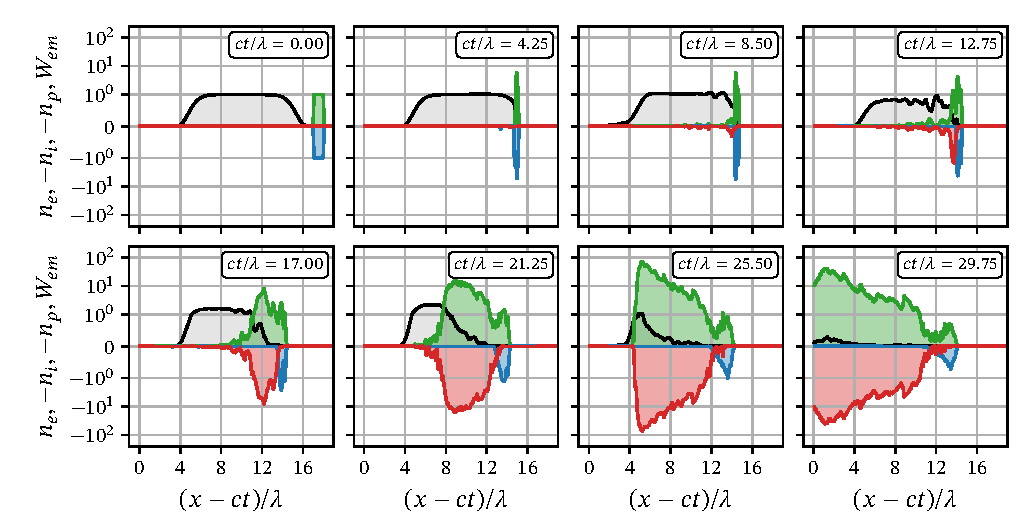
\includegraphics{cushion-onaxis.pdf}}
	\caption[Распределение плотности частиц и электромагнитной энергии в различные моменты времени в численном моделировании]{\label{Sim_res} Распределение плотности частиц (зелёная линия~---~электроны, синяя~---~ионы, красная~---~позитроны) и электромагнитной энергии (чёрная линия) вдоль оси $x$ в различные моменты времени. Значения нормированы на максимальные начальные значения. Масштаб вертикальной оси линейный для значений $[-1,1]$ и логарифмический для остальных значений.}
\end{figure}

\begin{figure}[h!]
	\centerfloat{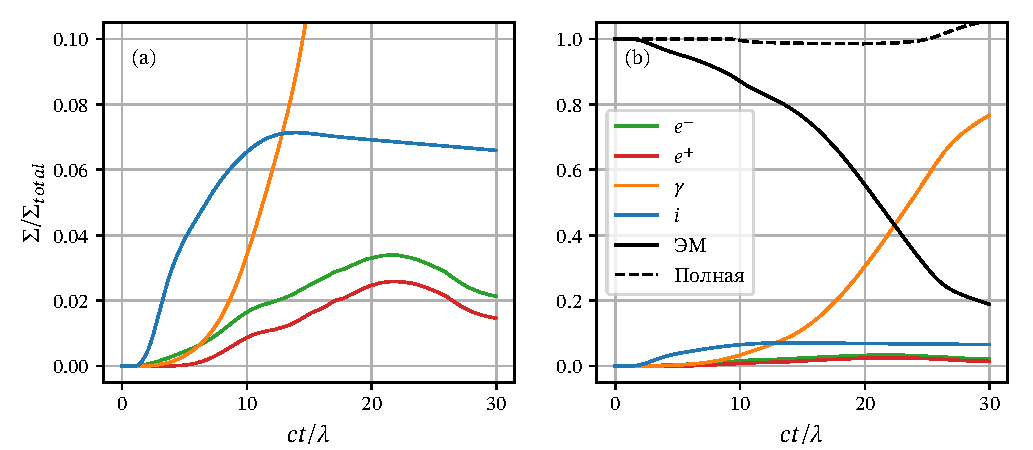
\includegraphics{cushion-energy.pdf} }
	\caption[Баланс энергии в системе в численном моделировании с параметрами $n_{e}=\SI{5.9e23}{\centi\meter^{-3}}$, $d=1$~мкм, $a_{0}=2500$]{\label{Sim_en} (a) Часть энергии лазерного импульса, перешедшая в энергию частиц, как функция времени. (b) Полная энергия системы, энергия лазерного импульса и энергия гамма-квантов, нормированные на начальное значение полной энергии.}
\end{figure}

Временная эволюция плотности частиц и электромагнитной энергии представлена на Рис.~\ref{Sim_res} для счёта с параметрами: ${n_{e}=\SI{5.9e23}{\centi\meter^{-3}}\approx530\, n_\mathrm{cr}}$ (${n_\mathrm{cr}=m_{e}\omega_{L}^{2}/4\pi e^{2}\approx\SI{1e21}{\centi\meter^{-3}}}$~---~критическая концентрация), $d=1$~мкм, $a_{0}=2500$. 
Из анализа результатов численного моделирования следует, что до времени $ct/\lambda\lesssim 8$ мишень сжимается в тонкий слой и ускоряется в продольном направлении до скорости, близкой к скорости света, т.е. происходит типичное ускорение ионов в режиме <<светового паруса>> (см. Рис.~\ref{Sim_en}\;(a)). 
Число электрон-позитронных пар, образованных в течение этого времени, незначительно. В интервал времени $8~\lesssim~ct/\lambda~\lesssim~14$ начинает формироваться неоднородная электрон-позитронная плазма, которая частично поглощает излучение, что приводит к снижению эффективности ускорения ионов (см. Рис.~\ref{Sim_en}\;(a)).
В период времени $14~\lesssim~ct/\lambda~\lesssim~28$ КЭД каскад развивается в самоподдерживающемся режиме, т.е. без участия частиц начальной затравки. 
При этом передний (по отношению к лазерному импульсу) фронт распределения электрон-позитронной пары движется со скоростью $v_\mathrm{fr}$ меньшей, чем скорость света; задний фронт при этом по инерции движется вместе с мишенью практически со световой скоростью. 
Таким образом электрон-позитронная подушка расширяется навстречу лазерному излучению и в конце концов полностью поглощает его. 
Такое поведение во многом напоминает распространение фронта ионизации при СВЧ пробое в газе \cite{semenov1982breakdown}.

\begin{figure}[h!]
	% \includegraphics[width=1\linewidth]{x_t2.pdf}
    \centerfloat{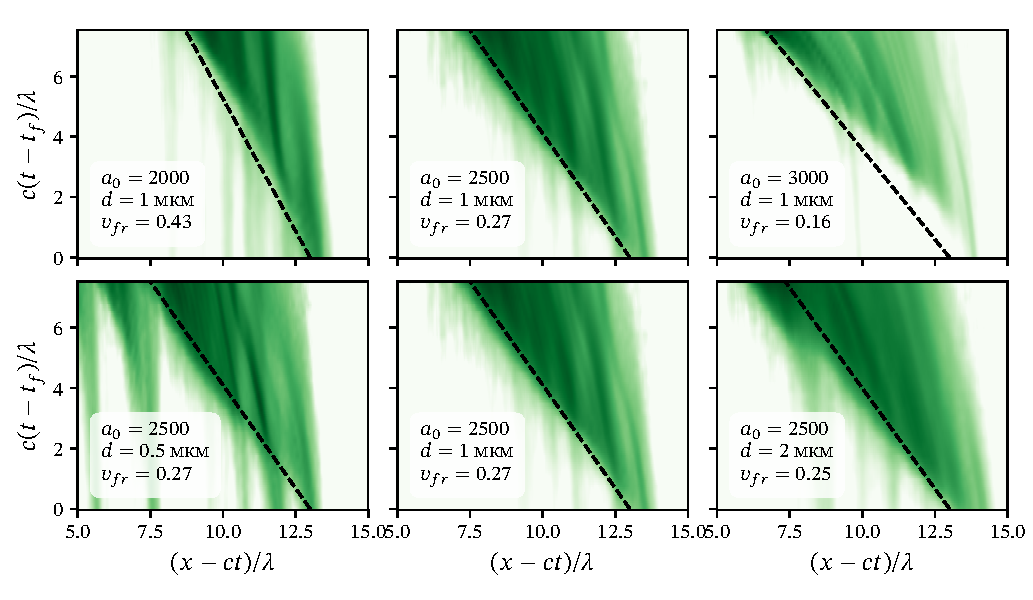
\includegraphics{cushion-xt.pdf}}
    \caption[Распределение позитронов в плоскости $x-t$ в численных моделированиях с различными начальными параметрами]{
        \label{fig:ch2/cushion-x-t}
        Распределение позитронов в плоскости $x-t$. Более яркий цвет обозначает большую плотность. Значения скорости фронта каскада (белые штриховые линии) даны в лабораторной системе отсчёта. $t_{f}$~---~приблизительное время начала образования подушки. $ct_{f}/\lambda\approx17.5$ для $a_{0}=2000$, $ct_{f}/\lambda\approx15.0$ для $a_{0}=2500$, $ct_{f}/\lambda\approx12.5$ для $a_{0}=3000$.}
\end{figure}

Мы провели ряд численных счётов с различными значениями $a_{0}=1500$, $2000$, $2500$, $3000$ и мишенью толщиной $d=1$~мкм и с различными значениями $d=0.5$~мкм, $1$~мкм, $2$~мкм для $a_{0}=2500$. 
На Рис.~\ref{fig:ch2/cushion-x-t} видно, что скорость фронта каскада слабо зависит от времени и толщины мишени, тогда как сильно зависит от интенсивности лазерного импульса, уменьшаясь (в лабораторной системе отсчёта) с её ростом. 
Также стоит отметить, что на поздних стадиях взаимодействия концентрация электрон-позитронной плазмы в несколько раз превышает значение релятивистской критической концентрации~$a_0 n_\mathrm{cr}$. 
Во всех проведённых счётах каскад эффективно развивается, однако, при $a_0=1500$ концентрация плазмы достигает значения $0.6 a_0 n_\mathrm{cr}$ к концу моделирования ($t = 30 \lambda/c$).
Поэтому мы предполагаем, что значение $a_0=1500$ грубо является пороговым значением для развития самоподдерживающегося каскада в плоской волне.

Для того, чтобы определить роль ионов мишени в образовании КЭД каскада, мы провели моделирование взаимодействия лазерного импульса с закритической электрон-позитронной мишенью. 
Геометрия мишени и импульса выбрана такой же, как описано выше. 
Толщина мишени составляла $d=1$~мкм, концентрация электронов $n_e = 0.7 a_0 n_\mathrm{cr}$, $a_0=2500$. 
Анализ результатов моделирования показывает, что самоподдерживающийся КЭД каскад развивается таким же образом, как и при затравке из электрон-ионной мишени; более того, совпадает и скорость фронта каскада. 
Из этого можно сделать вывод, что определённым выбором затравки и достаточно высокой интенсивностью лазерного импульса можно добиться развития КЭД каскада А-типа в поле с конфигурацией, близкой к плоской волне.

\begin{figure}[h!]
	\center{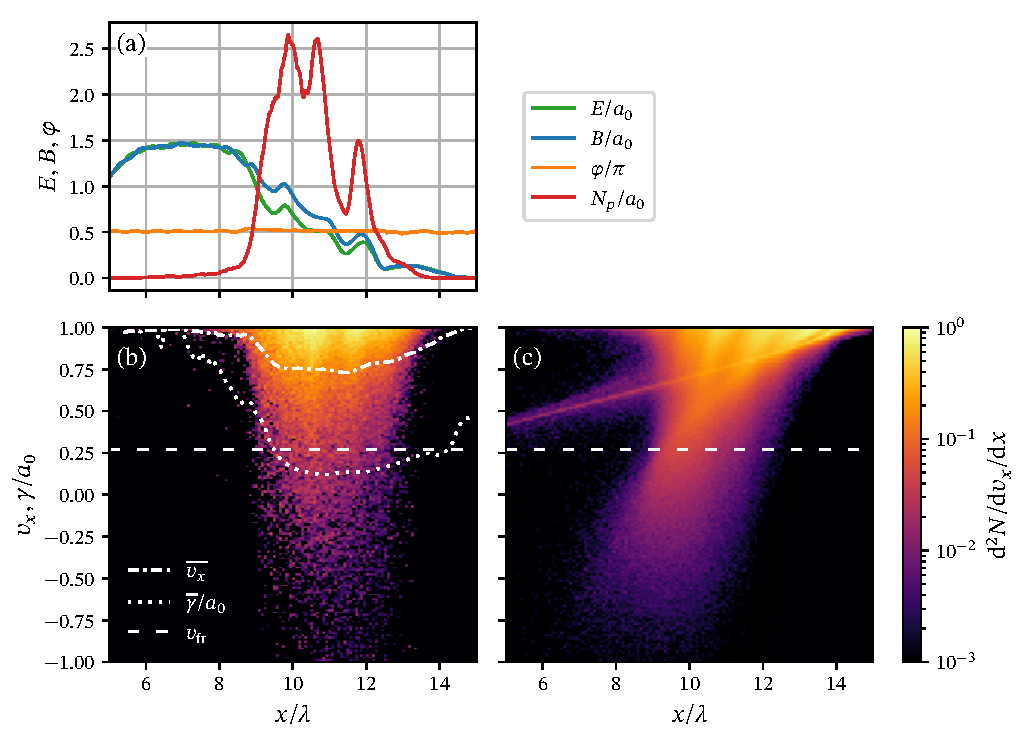
\includegraphics{cushion-fields-particles.pdf}}
    \caption[Результаты численного моделирования развития КЭД каскада в плоской волн]{\label{fig:ch2/field-structure} Результаты численного моделирования в момент времени ${t = 20 \lambda / c}$. (а) Распределение амплитуды электрического поля $E$, амплитуды магнитного поля $B$, угла $\varphi$ между ними и концентрации позитронов $N_p$. Распределение (b) позитронов ((с) гамма-квантов) в плоскости $x - v_{x}$ (плотность частиц обозначена цветом), их средние продольная скорость $\overline{v_x}$ (белая штрих-пунктирная линия) и Лоренц-фактор $\overline{\gamma}$ (белая пунктирная линия) как функции $x$. Белой штриховой линией обозначена скорость фронта каскада $v_\mathrm{fr}$ (равная 0.27 в данном моделировании).}
\end{figure}

\begin{figure}[h!]
	\center{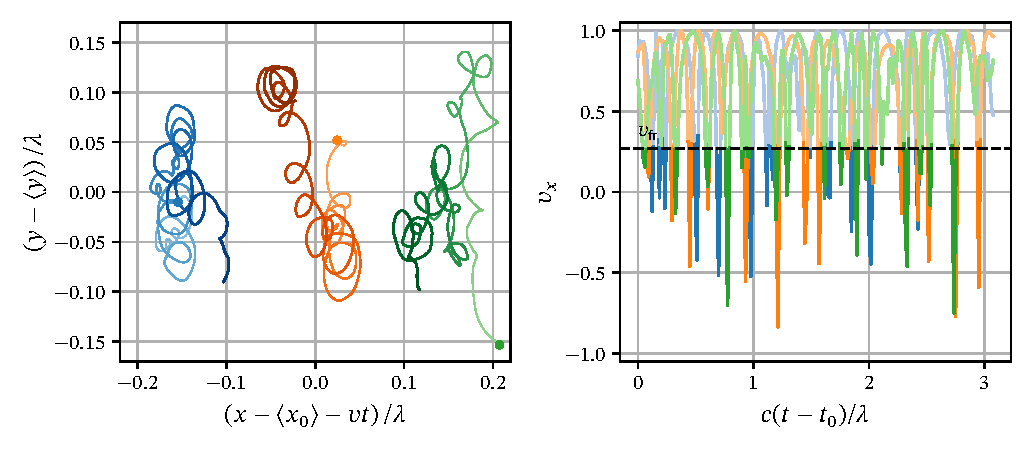
\includegraphics{cushion-tracks.pdf}}
    \caption[Характеристики движения отдельных электронов, находящихся внутри электрон-позитронной подушки.]{\label{fig:ch2/sec1/tracks} Характеристики движения трёх электронов, находящихся внутри электрон-позитронной подушки. (a) Траектории электронов в плоскости $xy$, в системе отсчёта, движущейся со скоростью $v=0.7$. Положение частицы в более поздние моменты времени обозначено более тёмным цветом, начальное положение частицы отмечено кружком. (b) Зависимость продольной скорости в зависимости от времени. Чёрная пунктирная линия соответствует скорости фронта каскада $v_\mathrm{fr} = 0.27$.}
\end{figure}

\subsection{Ключевые особенности и механизм развития КЭД каскада}
\label{sub:ch2/sec2/Mechanism}

Рассмотрим более подробно распределение электромагнитного поля и динамику частиц внутри электрон-позитронной плазмы для определения механизма развития каскада. 
Из Рис.~\ref{fig:ch2/field-structure}~(a) следует, что структура поля близка к циркулярно-поляризованной волне с перпендикулярными электрической и магнитной компонентами, $\vb{E \perp B}$, и поле затухает в плазме на масштабе в несколько длин волн. 
Ключевая особенность конфигурации поля~---~преобладание магнитного поля над электрическим, $B > E$.
В таком поле электроны и позитроны не набирают энергию (см. линию $\overline{\gamma} / a_0$ на  Рис.~\ref{fig:ch2/field-structure}~(b)), поэтому развитие каскада внутри плазмы подавлено.
Более того в таком поле траектории частиц представляют собой винтовые линии (см. Рис.~\ref{fig:ch2/sec1/tracks}~(a)). 
Это легко объясняется, если мы перейдём в систему отсчёта, движущуюся со скоростью $[\vb{E}~\times~\vb{B}]_x / B^2$, в которой электрическое поле параллельно магнитному и меньше его. 
В таком поле частицы вращаются в плоскости, перпендикулярной магнитному полю и могут иметь компоненту скорости вдоль магнитного поля. 
В лабораторной системе электроны и позитроны в среднем обгоняют фронт каскада, однако, из-за вращения частиц их мгновенная скорость вдоль оси $x$ иногда может быть меньше скорости фронта (см.  Рис.~\ref{fig:ch2/field-structure}~(b) и Рис.~\ref{fig:ch2/sec1/tracks}~(b)). 
В такие моменты частицы могут излучить гамма-квант, который попадёт в вакуумную область (большое количество гамма-квантов, распространяющихся медленнее фронта каскада и даже навстречу лазерному излучения, наблюдается в численном моделировании, что продемонстрировано на Рис.~\ref{fig:ch2/field-structure} (c)) и родит в сильном поле новую пару. 
Эта пара ускоряется сильным поле внутрь плазмы, где магнитное поле больше электрического и процесс повторяется.
Таким образом, самоподдерживающееся развитие каскада происходит на границе вакуума и подушки.
Важно подчеркнуть принципиальное различие между \textit{вакуумной} и \textit{плазменной} областями: в первой электромагнитная энергия передается каскадным частицам, а во второй частицы не ускоряются, а высвобождают полученную энергию в виде гамма-излучения.
Некоторая часть этого излучения возвращается обратно в область вакуума и обеспечивает положительную обратную связь, необходимую для поддержания каскада.
Механизм поддержания КЭД каскада в плоской волне схематически представлен на рисунке~\ref{fig:ch2/sec2/scheme}.

% \begin{figure}[h!]
% 	\center{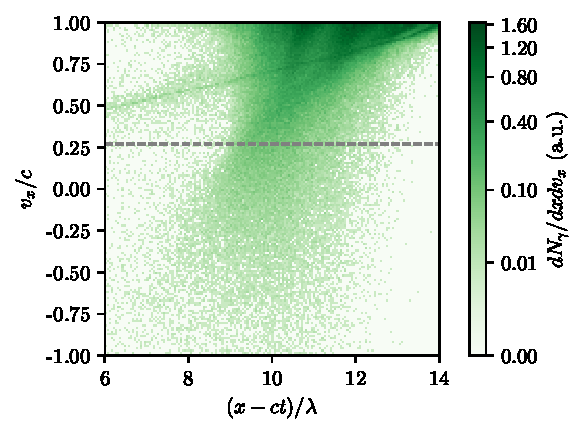
\includegraphics[width=100mm]{gamma2.pdf}}
% 	\caption{\label{gamma10} \fixme{Распределение гамма-квантов в плоскости $x - v_x$ в момент времени $t=20 \lambda /c $. Серая пунктирная линия обозначает скорость фронта $v_\mathrm{fr}$.} }
% \end{figure}


\begin{figure}[ht]
    \centerfloat{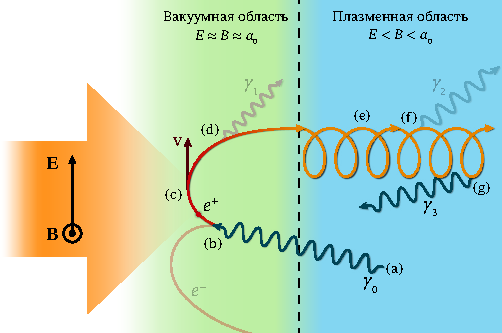
\includegraphics[width=155mm]{cushion-scheme.pdf}}
    \caption[Механизм поддержания КЭД каскада в плоской волне]{
    Схематическое изображение механизма поддержания КЭД каскада. (a), (f), (g) Излучение \textit{активного} (см. ниже) гамма-кванта в плазменной области, (b) распад \textit{активного} гамма-кванта в вакуумной области, (c) ускорение электрона и позитрона в плоской волне, (d) излучение \textit{пассивного} гамма-кванта в вакуумной области, (e) движение позитрона по винтовой линии в плазменной области.}
    \label{fig:ch2/sec2/scheme}
\end{figure}

\section{Аналитическое описание самоподдерживающегося КЭД каскада в плоской волне}
\label{sec:ch2/sec3}

Приступим к аналитическому описанию описанных выше процессов.
Аналогично работам~\cite{nerush2011analytical, elkina2011qed} запишем кинетические уравнения для электронов, позитронов и гамма-квантов, предполагая, что КЭД каскад находится на стадии самоподдержания, поэтому затравочные частицы, например, электроны и ионы начальной мишени, не влияют на его развитие.
Кинетические уравнения совместно с уравнениями Максвелла (в виде теоремы Пойнтинга) записываются в следующем виде
\begin{align}
    \label{eq:ch2/Boltzman1}
    \pdv{f_{e^\pm}}{t} +  \vb{v}_{e^\pm} \nabla f_{e^\pm} \pm \left( \vb{E} + [\vb{v}_{e^\pm} \times \vb{B}] \right) \pdv{ f_{e^\pm}}{ \vb{p}} \ &
    \begin{aligned}[t]
        = & \int f_\gamma(\vb{p'}) w_\mathrm{pair}(\vb{p', p}) \dd\vb{p'} + \\
        + & \int f_{e^\pm}(\vb{p'}) w_\mathrm{rad}(\vb{p', p}) \dd\vb{p'} - \\
        - & \int f_{e^\pm}(\vb{p}) w_\mathrm{rad}(\vb{p, p'}) \dd\vb{p'}  ,
    \end{aligned} \\
    \label{eq:ch2/Boltzman2}
    \pdv{f_\gamma}{t} + \vb{v}_\gamma\nabla f_\gamma \ &
    \begin{aligned}[t]
        = &\int  f_{e^\pm}(\vb{p'}) w_\mathrm{rad}(\vb{p', p'-p}) \dd\vb{p'} - \\ 
        + &\int f_\gamma(\vb{p}) w_\mathrm{pair}(\vb{p, p'}) \dd\vb{p'} ,
    \end{aligned} \\
    \label{eq:ch2/Max1}
    \pdv{}{t}\left( \frac{E^2 + B^2}{2} \right) + \nabla [\vb{E}\times\vb{B}] &= \int f_{e^-}(\vb{p}) (\vb{v}_{e^-} \vb{E}) \dd\vb{p} - \\
    &- \int f_{e^+}(\vb{p}) (\vb{v}_{e^+}\vb{E}) \dd\vb{p} ,
    % \frac{\partial \vb{B}}{\partial t} + \nabla\times \vb{E} &= 0, \\
    % \label{eq:ch2/Max2}
    % \frac{\partial \vb{E}}{\partial t} - \nabla\times \vb{B} &=  \int f_{e^-} \vb{v}_{e^-} \dd\vb{p} -  \int f_{e^+} \vb{v}_{e^+} d\vb{p} ,
\end{align}
где $f_{e^\pm,\gamma}(t,\vb{r,p})$~---~функции распределения электронов, позитронов и гамма-квантов соответственно, $\vb{v}$~---~скорость частиц, равная $\vb{p}/\sqrt{1+p^2}$ для электронов и позитронов и равная $\vb{p}/p$ для гамма-квантов, $w_\mathrm{rad}(\vb{p', p})\dd\vb{p'}$~---~вероятность излучения электроном или позитроном с импульсом $\vb{p'}$ гамма-кванта с импульсом $\vb{p'-p}$ в единицу времени, $w_\mathrm{pair}(\vb{p', p})\dd\vb{p'}$~---~вероятность распада гамма-кванта с импульсом $\vb{p'}$ на электрон с импульсом $\vb{p}$ и позитрон с импульсом $\vb{p'-p}$ в единицу времени.
Здесь также используется уже описанная выше релятивистская нормировка, при которой электрическое и магнитное поля нормируются на величину $m_ec\omega_\mathrm{L}/e$, концентрация частиц~---~на критическую концентрацию $n_\mathrm{cr}=m_e\omega_\mathrm{L}^2/4\pi e^2$, энергия и импульс~---~на $m_e c^2$ и $m_e c$ соответственно, координаты и время~---~на $c/\omega_\mathrm{L}$ и $1/\omega_\mathrm{L}$ соответственно.

\subsection{Предположения модели}
\label{sub:ch2/sec3/Assumptions}
Применим ряд упрощений к записанным выше уравнениям.
Во-первых, т.к. исследуется взаимодействие с плоской ЭМ волной, то будем считать задачу пространственно одномерной.
Более того, будем рассматривать взаимодействие с циркулярно-поляризованной волн, что приводит к симметрии относительно поворота вдоль оси распространения волны (для определённости оси $x$ здесь и далее).
Данные предположения приводят к тому, что функции распределения частиц становятся зависимыми только от трёх переменных (исключая время) вместо шести, т.е. $f(t;\vb{r},\vb{p})=f(t;x,p,\theta)/2\pi$, где $p$~---~импульс частицы, $\theta$~---~угол между вектором импульса частицы и осью симметрии $x$.

Во-вторых, предположим, что функции распределения являются локально моноэнергитическими, т.е. $f\propto\delta(p-\overline{p}(x))/p^2$, где $\overline{p}(x)$~---~среднее значение импульса частиц, расположенных в малой окрестности $x$.
Обозначим среднюю энергию гамма-квантов как $\varepsilon_\gamma$, и среднюю энергию электрон-позитронных пар как $\varepsilon_p$, предполагая, что они ультрарелятивистские, поэтому $\varepsilon_p^2 = 1+p_p^2\approx p_p^2$.
Несмотря на то, что моноэнергитическое приближение является сильно упрощающим, мы предполагаем, что механизм развития и КЭД каскада, описанный выше, принципиально не зависит от каких-либо особенностей спектра частиц.
Поэтому мы утверждаем, что учет эволюции энергетических спектров в нашей модели вызовет только количественные, а не качественные изменения, при этом сильно усложняя уравнения.
Как будет показано ниже, это предположение справедливо для пар, которые попадают в область плотной электрон-позитронной плазмы с примерно равными энергиями.
Для гамма-квантов мы используем двухпотоковое приближение, т.е. разделяем гамма-кванты на те, которые излучаются в вакуумной области и распространяются в основном вдоль направления распространения лазерного импульса и, таким образом, не дают вклада в развитие каскада (мы обозначим их как \textit{пассивные} гамма-кванты) и те, которые излучаются в области плазмы в различных направлениях и обеспечивают положительную обратную связь, необходимую для развития каскада (мы обозначаем их либо как \textit{активные} гамма-кванты, либо просто гамма-кванты).
Как видно из Рис.~\ref{fig:ch2/sec3/gamma_energy} энергетический спектр гамма-квантов является достаточно широким, однако если исключить пассивные гамма-кванты, то ширина спектра значительно уменьшается, что оправдывает наше предположение.
Поскольку пассивные гамма-кванты влияют на развитие каскада только забирая часть общей энергии, их пространственное распределение не имеет значения для развития каскада, однако оно всё равно будет рассчитано для более точного сравнения с результатами QED-PIC моделирования.

\begin{figure}[ht]
    \centerfloat{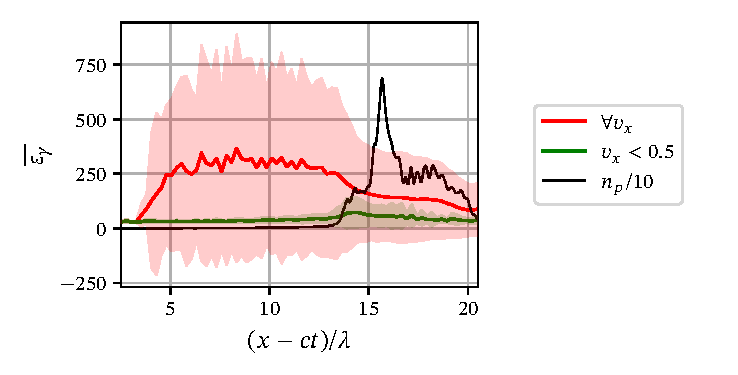
\includegraphics{cushion-gamma-energy}}
    \caption[Сравнение ширины разброса энергий всех гамма-квантов и только активных гамма-квантов]{\label{fig:ch2/sec3/gamma_energy} 
    Средняя энергия $\varepsilon_\gamma$ гамма-квантов в зависимости от координаты $x$, рассчитанная по всем частицам (красная линия) и только по частицам со скоростью вдоль оси  $x$ не превышающей 0.5, что по нашим предположениям включает только активные гамма-кванты (зелёная линия). Закрашенные цветные области отображают среднеквадратичное отклонение энергии. Данные взяты из результатов PIC моделирования в момента времени $ct/\lambda=18$. Параметры моделирования обсуждаются в подразделе~\ref{sub:ch2/sec3/Numeric}. Начальные условия такие же, как на Рис.~\ref{fig:ch2/sec3/sol2500}. Чёрная линия соответствует распределению плотности электрон-позитронной плазмы.}
\end{figure}

Для того, чтобы опустить интегрирование по энергиям и азимутальному углу $\varphi$ (в плоскости $yz$), переопределим функции распределения $f$ следующим образом
\begin{equation}
    f(x, \varepsilon, \theta, \varphi) \rightarrow \int\limits_0^\infty\int\limits_0^{2\pi}f(x,\varepsilon,\theta,\varphi)2\pi\varepsilon^2\dd\varphi \dd\varepsilon = n(x)\Phi(\theta),
\end{equation}
где $n(x)$~---~концентрация частиц, $\Phi(\theta)$~---~функция распределения импульса частиц по углу $\theta$, причём
\begin{align}
    \int\limits_{-\infty}^{+\infty} n(x)\dd x = N, \\
    \int\limits_0^\pi \Phi(\theta)\sin\theta \dd\theta = 1,
\end{align}
где $N$~---~полное число частиц.

Предположение о моноэнергитичности фактически соответствует переходу от кинетического к гидродинамическому описанию, т.е. записи уравнений на моменты функций распределения.
Чтобы записать гидродинамические уравнения предварительно введём несколько дополнительных величин
\begin{align}
    \label{eq:ch2/Wpair0}
    W_\mathrm{pair}(\chi_\gamma, \varepsilon_\gamma) = \int w_\mathrm{pair}(\vb{p},\vb{p'})\dd\vb{p'} ,\\
    \label{eq:ch2/Wrad0}
    W_\mathrm{rad}(\chi_p, \varepsilon_p) = \int w_\mathrm{rad}(\vb{p},\vb{p'})\dd\vb{p'} ,\\
    \label{eq:ch2/Irad0}
    I_\mathrm{rad}(\chi_p) = \int w_\mathrm{rad}(\vb{p},\vb{p'})(\varepsilon_p-\varepsilon_p')\dd\vb{p'},
\end{align}
где $W_\mathrm{pair}, W_\mathrm{rad}, I_\mathrm{rad}$~---~полная вероятность фотообразования электрон-позитронных пар, полная вероятность и мощность излучения гамма-квантов соответственно~\cite{Baier98}. 
Как неоднократно указывалось выше, данные величины зависят от Лоренц-инвариантного КЭД параметра $\chi$
\begin{equation}
    \chi = \frac{\varepsilon}{a_\mathrm{S}} \sqrt{ \left(\vb{E}+\vb{v}\times\vb{B}\right)^{2}-\left(\vb{v}\cdot\vb{E}\right)^{2} } ,
\end{equation}
где $\varepsilon$~---~энергия частицы, $a_\mathrm{S} = e E_\mathrm{S}/m_ec\omega_\mathrm{L} = m_ec^2/\hbar\omega_\mathrm{L}$ и $a_\mathrm{S}={m_e}^2c^3/\hbar e$~---~поле Заутера-Швингера~\cite{berestetskii1982quantum}.
В общем виде гидродинамические уравнения выглядят как уравнения переноса (непрерывности)
\begin{equation}
    \pdv{ D_\alpha}{ t} + \pdv{ F_\alpha}{ x} = \sum_{\beta} S[\alpha, \beta] ,
\end{equation}
где $D_\alpha$ и $F_\alpha$~---~плотность и поток некоторой физической величины $\alpha$, $S[\alpha,\beta]$~---~источник, приводящий к изменению величины $\alpha$ в результате процесса $\beta$.
Отметим, что несмотря на то, что мы определили функцию распределения частиц по энергиям, для вычисления источников $S[\alpha,\beta]$ также необходимо знать угловое распределение частиц, которое обсуждается ниже.
Основываясь на качественном объяснении механизма развития и поддержания КЭД каскада, описанном в подразделе~\ref{sub:ch2/sec2/Mechanism}, мы предполагаем, что следующая система уравнений достаточно полно описывает данный процесс 
\begin{align}
    \label{eq:ch2/hd_p1}
    \frac{\partial }{\partial t}n_p  \quad &\!+\!& &\frac{\partial}{\partial x}\left( v_x n_p \right) \!\!\!&\!&\!=  S[n, \mathrm{pp}] ,\\
    \label{eq:ch2/hd_p2}
    \frac{\partial}{\partial t}\left( \varepsilon_p n_p \right)   \quad &\!+\!& & \frac{\partial}{\partial x}\left( v_x \varepsilon_p n_p \right) \!\!\!&\!&\!=
    \begin{aligned}[t]
        & S[\varepsilon, \mathrm{pp}] + S[\varepsilon, \mathrm{\mathrm{acc}}] \psi_\mathrm{vac} - \\
        & - S[\varepsilon, \mathrm{rad_a}] \psi_\mathrm{pl} - S[\varepsilon, \mathrm{rad_p}] \psi_\mathrm{vac} ,
    \end{aligned} \\
    \label{eq:ch2/hd_g1}
    \frac{\partial }{\partial t}n_\gamma  \quad &\!+\!& &\frac{\partial}{\partial x}\left( \overline{v_{\gamma\parallel}} n_\gamma \right)\!\!\!&\!&\!= -S[n, \mathrm{pp}] + 2 S[n, \mathrm{rad_a}] \psi_\mathrm{pl} ,\\
    \label{eq:ch2/hd_g2}
    \frac{\partial}{\partial t}\left( \overline{v_{\gamma\parallel}} n_\gamma \right) \quad &\!+\!& & \frac{\partial}{\partial x}\left( \overline{v_{\gamma\parallel}^2} n_\gamma \right) \!\!\!&\!&\!=  -S[v, \mathrm{pp}] + 2 S[v, \mathrm{rad_a}] \psi_\mathrm{pl} ,\\
    \label{eq:ch2/hd_g3}
    \frac{\partial}{\partial t}\left( \varepsilon_\gamma n_\gamma \right) \quad &\!+\!& &\frac{\partial}{\partial x}\left( \overline{v_{\gamma\parallel}} \varepsilon_\gamma n_\gamma \right) \!\!\!&\!&\!= -S[\varepsilon, \mathrm{pp}] + 2 S[\varepsilon, \mathrm{rad_a}] \psi_\mathrm{pl} ,\\
    \label{eq:ch2/hd_e1}
    \frac{\partial }{\partial t}\left( \frac{E^2 + B^2}{2} \right) \quad &\!+\!& &\frac{\partial}{\partial x} {\left[ \vb{E\times B} \right]}_x \!\!\!&\!&\!= - 2 S[\varepsilon, \mathrm{\mathrm{acc}}]\psi_\mathrm{vac} \equiv - \vb{jE} ,\\
    && & \qquad\quad \frac{\partial \Sigma_\gamma}{\partial t} \!\!\!&\!&\!= 2 \int\limits_0^\infty S[\varepsilon, \mathrm{rad_p}]\psi_\mathrm{vac} dx ,
\end{align}
где $n_p = n_{e^+} = n_{e^-}$~---~половина концентрации электрон-позитронной плазмы в предположении её квазинейтральности, $v_x$~---~средняя продольная скорость пар, рассчитываемая в подразделе~\ref{sub:ch2/sec3/fields}, $\overline{v_{\gamma\parallel}}$ и $\overline{v_{\gamma\parallel}^2}$~---~средняя величина и средний квадрат величины продольной скорости гамма-квантов.
Последние рассчитываются из углового распределения следующим образом
\begin{align}
    \overline{v_{\gamma\parallel}} = \int_0^\pi \Phi(\theta)\cos\theta\sin\theta d\theta, \\
    \overline{v_{\gamma\parallel}^2} = \int_0^\pi \Phi(\theta)\cos^2\theta\sin\theta d\theta.
\end{align}
Уравнение~\eqref{eq:ch2/hd_e1} является записью теоремы Пойнтинга, и которое фактически является уравнением переноса плотности электромагнитной энергии.
Источники $S[n,\beta]$, $S[v,\beta]$ и $S[\varepsilon,\beta]$ соответствуют изменению концентрации, продольной скорости и энергии частиц соответственно, источники $S[\alpha, \mathrm{pp}]$, $S[\alpha, \mathrm{acc}]$, $S[\alpha, \mathrm{rad_a}]$ и $S[\alpha, \mathrm{rad_p}]$ соответствуют процессам фотообразования пар, ускорения пар в плоской волне, излучению активных гамма-квантов парами в плазменной области и излучению пассивных гамма-квантов парами в вакуумной области соответственно (отмечены соответственно буквами (b), (c), (d) и (f) на Рис.~\ref{fig:ch2/sec2/scheme}), $\Sigma_\gamma$~---~полная энергия пассивных гамма-квантов.
Множитель $\psi_\mathrm{vac}(\psi_\mathrm{pl})$ считается равным 1 в вакуумной (плазменной) области и 0 в плазменной (вакуумной) области.
Вычисление данных множителей будет приведено ниже.
Отметим, что $\psi_\mathrm{vac}+\psi_\mathrm{pl}=1$.
Для удобства будем опускать дынные множители, когда рассматриваемая область очевидна.

\subsection{Конфигурация электромагнитного поля}
\label{sub:ch2/sec3/fields}

Согласно результатом трёхмерного QED-PIC моделирования электрическое и магнитное поля в плазменной области остаются практически перпендикулярными друг другу, а величина магнитного поля всюду превосходит величину электрического: $B > E$.
Пространственное распределение ЭМ поля имеет характерный масштаб $\lambda$ как в вакуумной, так и в плазменной области.
В таком поле заряженные частицы дрейфуют в направлении перпендикулярном, как электрическому, так и магнитному полю, т.е. вдоль оси $x$ со скоростью
\begin{equation}
    \label{eq:ch2/vdrift}
    v_x\approx E/B.
\end{equation}
В вакуумной области ЭМ поле представляет собой поле падающей плоской волны.
В таком случае электрическое и магнитное поля взаимно перпендикулярны и равны друг другу по величине.
Если энергия $\varepsilon$ частицы, попавшей в вакуумную область, меньше безразмерной амплитуды поля $E$, то согласно построенной в первой главе асимптотической теории за время, много меньшее периода волны, такая частица ускорится в продольном направлении практически до скорости света.
Таким образом можно считать, что в вакуумной области выполняется соотношение $v_x\approx 1=E/B$, т.е. уравнение~\eqref{eq:ch2/vdrift} в действительности справедливо как в плазменной, так и в вакуумной области.

В данном рассуждении мы не учитываем отражённую от границы $e^-e^+$ плазмы волну по нескольким причинам.
Во-первых, в трёхмерном QED-PIC моделировании не наблюдается существенного отражения при развитии каскада на стадии его самоподдержания.
Во-вторых, отражение, возникающее на начальном этапе лазерного взаимодействия с тонкой твердой мишенью, согласно теории относительности, быстро истощается по мере ускорения частиц в направлении распространения лазерного импульса и, таким образом, становится несущественным для более поздних стадий развития каскада.
Однако наша модель не описывает электрон-ионную плазму, поэтому мы исследуем взаимодействие лазерного импульса с затравкой в виде встречного гамма-сгустка (см. подраздел~\ref{sub:ch2/sec3/Numeric}), где отражения не происходит даже на начальном этапе взаимодействия.
Кроме того, отражение незначительно изменило бы процесс фоторождения пар в связи с тем, что наибольшей вероятностью распада обладают гамма-кванты, распространяющиеся навстречу лазерному импульсу, т.е. попутно отраженному излучению.
А поля попутной волны не увеличивают значение определяющего КЭД-параметра $\chi$ гамма-квантов.
Наконец, в вакуумной области, где лазерное поле наиболее сильное, находятся в основном ультрарелятивистские электроны и позитроны, образованные из фотонов с наиболее высокой энергией.
Рассеяние релятивистски сильного лазерного поля ($a_0 \gg 1$) на ультрарелятивистских электронах и позитронах ($\gamma \gg 1$) происходит как в нелинейном, так и в квантовом режиме.
Из-за этого, а также из-за того, что положение частиц нескоррелировано, результирующее рассеянное излучение некогерентно и его частота сильно сдвинута вверх.
Такое излучение лучше всего описывается отдельными фотонами, как это и реализовано в коде QUILL.
Часть этих фотонов, распространяющихся навстречу лазерному импульсу, действительно можно рассматривать как отражение.
Хотя такие фотоны могут увеличить общий выход электрон-позитронных пар и гамма-квантов за счет КЭД процессов более высокого порядка, они значительно менее вероятны, чем нелинейное комптоновское рассеяние и процесс Брейта-Уилера, и поэтому не учитываются ни в QED-PIC моделировании, ни в нашей модели.
Отметим, однако, что в нашей модели учитываются потери энергии из-за некогерентного гамма-излучения как в вакуумной, так и в плазменной областях.

\subsection{Функция распределения активных гамма-квантов}
\label{sub:ch2/sec3/gammas}

Как описано в разделе~\ref{sub:ch2/sec2/Mechanism} активные гамма-кванты излучаются парами в процессе их движения по винтовым траекториям в плазменной области.
В связи с этим их угловое распределение является широким.
Предположим также, что это распределение плавное и может быть описано всего одним параметром.
Данным параметром является скорость $v$ мгновенной системы отсчёта $K'$, в которой угловое распределение фотонов, находящихся вблизи малой окрестности координаты $x$, является практически изотропным, т.е.
\begin{equation}
    \Phi'(\theta') \equiv \frac{\dd N'}{\dd \cos\theta'} = \frac{1}{2},
\end{equation}
где $\dd N'=\dd N$~---~число частиц с продольной скоростью в диапазоне $[\cos\theta', \cos\theta'+\dd\cos\theta']$ и
\begin{equation}
    \cos\theta' = \frac{\cos\theta - v}{1 - v \cos\theta}.
\end{equation}
В лабораторной системе отсчёта такое распределение выглядит следующим образом~\cite{LandauII}
\begin{equation}
    \label{eq:ch2/Phi}
    \Phi(\theta, v) = \frac{\dd N}{\dd \cos\theta} = \frac{\dd N'}{\dd \cos\theta'} \frac{\dd \cos\theta'}{\dd \cos\theta} = \frac{1-v^2}{{2\left( 1 - v \cos{\theta}  \right)}^2}.
\end{equation}
Таким образом, функция распределения активных гамма-квантов имеет следующий вид
\begin{equation}
    f_\gamma(t; x,\theta)=\Phi\left(\theta, v_{\gamma\parallel}(x,t)\right) n_\gamma(x,t).
\end{equation}
Средняя величина $\overline{v_{\gamma\parallel}}$ и средний квадрат величины $\overline{v_{\gamma\parallel}^2}$ продольной скорости рассчитываются следующим образом
\begin{align}
    \label{eq:ch2/av_vx}
    \overline{v_{\gamma\parallel}}=\int_0^\pi \Phi(\theta, v) \cos{\theta} \sin{\theta}\dd\theta = \frac{1}{v_{\gamma\parallel}} - \frac{1-v_{\gamma\parallel}^2}{v_{\gamma\parallel}^2}\text{ath}(v_{\gamma\parallel}) , \\
    \overline{v_{\gamma\parallel}^2}=\int_0^\pi \Phi(\theta, v) \cos^2{\theta} \sin{\theta}\dd\theta = \frac{2\overline{v_{\gamma\parallel}}}{v_{\gamma\parallel}} - 1 ,
\end{align}
где $\text{ath}(x)$~---~обратная функция гиперболического тангенса.
Отметим, что согласно преобразованиям Лоренца средняя скорость гамма-квантов $\overline{v_{\gamma\parallel}}$ отличается от скорости $v_{\gamma\parallel}$ системы отсчёта $K'$, в которой их распределение изотропно.
Результаты QED-PIC моделирования показывают, что выражение~\eqref{eq:ch2/Phi} является достаточно хорошей аппроксимацией углового распределения активных гамма-квантов (см. Рис.~\ref{fig:ch2/sec3/ang} (a), (b)).

\begin{figure}[ht]
    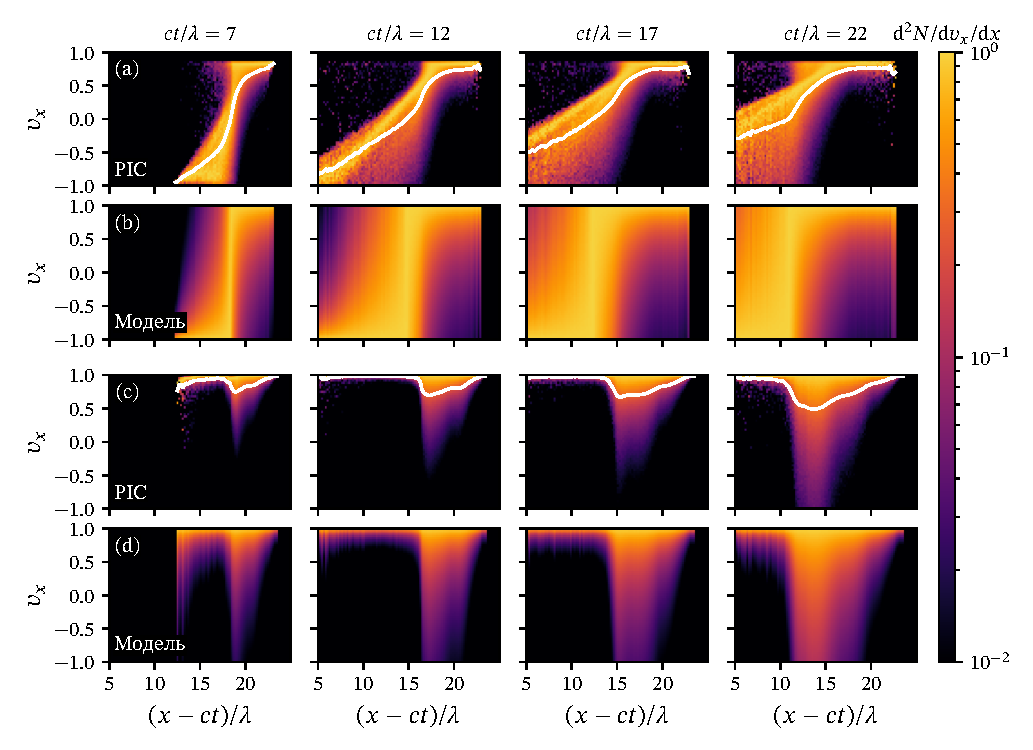
\includegraphics{cushion-ang-new.pdf}
    \caption[Проверка приближения, использованного для описания углового распределения частиц.]{\label{fig:ch2/sec3/ang}
    Проверка приближения, использованного для описания углового распределения частиц. Угловое распределение частиц ((a)~---~гамма-квантов, (c)~---~$e^-e^+$ пар), расположенных в малой окрестности координаты $x$ (цветовая карта) и их средняя продольная скорость, рассчитанная по этому распределению (белая линия) согласно результатам численного QED-PIC моделирования. (b), (d)~---~модельное угловое распределение гамма-квантов и $e^-e^+$ пар соответственно, восстановленное по средней скорости с помощью выражения~\eqref{eq:ch2/Phi}. }
\end{figure}

Значение величины КЭД параметра $\chi$ для гамма-квантов, находящихся в скрещенных электрическом и магнитном полях, что справедливо как для вакуумной, так и для плазменной области, вычисляется следующим образом
\begin{equation}
    \chi_\gamma = \frac{\varepsilon_\gamma \left| B - E\cos\theta \right|}{a_\mathrm{S}} = \frac{\varepsilon_\gamma E }{a_\mathrm{S}}\frac{1- v_x\cos\theta }{v_x},
\end{equation}
где было использовано выражение~\eqref{eq:ch2/vdrift}.

Полностью определив функцию распределения гамма-квантов, можно вычислить источники $S[\alpha, \mathrm{pp}]$, соответствующие процессу фоторождения пар
\begin{align}
    S[n,\mathrm{pp}] =  n_\gamma\int\limits_0^\pi \Phi(\theta, v_{\gamma\parallel}) W_\mathrm{pair}(\chi_\gamma,\varepsilon_\gamma) \sin\theta \dd\theta \equiv \overline{W_\mathrm{pair}} n_\gamma , \\
    S[\varepsilon,\mathrm{pp}] = \varepsilon_\gamma n_\gamma\int\limits_0^\pi \Phi(\theta, v_{\gamma\parallel}) W_\mathrm{pair}(\chi_\gamma,\varepsilon_\gamma) \sin\theta \dd\theta \equiv \overline{W_\mathrm{pair}} \varepsilon_\gamma n_\gamma ,\\
    S[v,\mathrm{pp}] = n_\gamma\int\limits_0^\pi \Phi(\theta, v_{\gamma\parallel}) W_\mathrm{pair}(\chi_\gamma,\varepsilon_\gamma)\cos\theta \sin\theta \dd\theta \equiv \overline{V_\mathrm{pair}} n_\gamma .
\end{align}

\subsection{Динамика $e^-e^+$ пар в вакуумной области}
Рассмотрим электроны и позитроны, образовавшиеся в вакуумной области, где их число настолько мало, что коллективными плазменными эффектами можно пренебречь, поэтому ЭМ поле в данной области представляет собой поле падающей плоской волны. 
Динамика единичного электрона в поле экстремально интенсивной плоской волны подробно рассмотрено в подразделе~\ref{sub:ch1/sec6/CPW} данной работы.
Как упоминалось выше, для вычисления источников $S[\alpha, \beta]$ в правой части уравнений~\eqref{eq:ch2/hd_p1}~--~\eqref{eq:ch2/hd_e1} необходимо знание углового распределения частиц.
Несмотря на то, что траектории электронов в плоской волне находятся аналитически, явное вычисление функции распределения по этим траекториям является фактически невозможным, т.к. частицы рождаются в этой области в случайные моменты времени с различными начальными условиями.
Однако, следующие рассуждения позволяют рассчитать источники $S[\alpha, \beta]$, исходя из другого подхода.
Во-первых, в очередной раз отметим, что релятивистски сильная плоская волна <<толкает>> частицы в направлении своего распространения, т.е. в нашем случае вдоль оси $x$.
Поэтому вне зависимости от начальных условий за короткий промежуток времени импульс частицы ориентируется практически вдоль оси $x$, и в вакуумной области мы считаем $v_x \approx 1$.
Пренебрегая временем такой ориентации, можно приближенно вычислить поток частиц и энергии путём умножения плотности этих величин на скорость $v_x \approx 1$.
Так как в вакуумной области по определению нет коллективных эффектов и в ней не развивается КЭД каскад, то уравнения непрерывности в этой области фактически служат лишь для того, чтобы рассчитать потоки частиц и энергии (включая электромагнитную) на фронте каскада в плазменную область.
Таким образом, нам необходимо знать лишь суммарный вклад в эти потоки от каждой частицы за время от момента её образования в вакуумной области до достижения границы с плазмой.
В связи с этим, источники $S[\varepsilon,\beta]$ можно вычислить следующим образом
\begin{equation}
    S[\varepsilon,\beta] = \int_0^\pi f_\gamma(x, \theta) W_\mathrm{pair}(\chi_\gamma, \varepsilon_\gamma) \Delta\varepsilon_\beta \sin\theta d\theta ,
\end{equation}
где $\Delta\varepsilon_\beta$~---~суммарное изменение энергии в процессе $\beta$ частицы, образовавшейся в точке с координатой $x$ в момент времени $t$, за всё время её нахождения в плазменной области.
Определяя источник $S[\varepsilon,\beta]$ таким образом, мы фактически считаем, что частица приобретает изменение энергии $\Delta\varepsilon_\beta$ в момент рождения, а затем без изменения энергии движется со скоростью света до плазменной области.

Для вычисления изменения энергии частицы при движении в циркулярно-поляризованной плоской волне воспользуемся результатами раздела~\ref{sub:ch1/sec6/CPW}.
\begin{equation}
    \label{eq:ch2/sec3/pw_vac}
    \Delta\varepsilon_\mathrm{acc} = \frac{2 E p_0}{p_{-, 0}} \sin\frac{\Delta\varphi}{2} \left( \frac{E}{p_0}\sin\frac{\Delta\varphi}{2} - \sin\theta\sin\frac{\varphi+\varphi_0}{2} \right),
\end{equation}
где мы не учитываем поправки, связанные с реакцией излучения, которые сказываются на большом числе периодов волны.
Так как частицы рождаются в произвольный момент времени и мы считаем распределение частиц по азимутальному углу изотропным, то выражение~\eqref{eq:ch2/sec3/pw_vac} необходимо усреднить по $\varphi_0$.
В таком случае получим
\begin{equation}
    \label{eq:ch2/sec3/pw_vac_av}
    \Delta\varepsilon_\mathrm{acc} = \frac{2 E^2}{p_{-, 0}} \sin^2\frac{\Delta\varphi}{2}.
\end{equation}
Для определения величины $\Delta\varepsilon_\mathrm{acc}$ необходимо вычислить время нахождения частиц в вакуумной области.
Для этого будем искать величину $\Delta\varphi$ из условия достижения продольной скорости частиц $v_x$ некого порогового значения $v_\mathrm{th}$, близкого к 1. 
В таком случае, после достижения этого порогового значения величина $\Delta\varphi$ и соответственно $\Delta\varepsilon_\mathrm{acc}$ практически не изменяются.
Запишем данное условие следующим образом
\begin{equation}
    v_\mathrm{th} = v_x = \frac{p_x}{\gamma} = \frac{\gamma - p_-}{\gamma_0 + \Delta\varepsilon_\mathrm{acc}} \approx \frac{p_{x,0} + \Delta\varepsilon_\mathrm{acc}}{\gamma_0 + \Delta\varepsilon_\mathrm{acc}} \approx \frac{\gamma_0 \cos\theta + \Delta\varepsilon_\mathrm{acc}}{\gamma_0 + \Delta\varepsilon_\mathrm{acc}},
\end{equation}
где в предпоследнем равенстве использовался факт, что $p_- = \text{const} = \gamma_0 - p_{x,0}$ без учёта реакции излучения, а в последнем~---~предполагалось, что $\gamma_0 \gg 1$, поэтому $p_0 = \sqrt{\gamma_0^2 - 1}\approx\gamma_0$.
Рассматривая данное выражение как уравнение на величину $\Delta\varepsilon_\mathrm{acc}$, получим
\begin{equation}
    \label{eq:ch2/sec3/deltae}
    \Delta\varepsilon_\mathrm{acc} = 2 \gamma_0 \gamma_\mathrm{th}^2 (1 - \cos\theta),
\end{equation}
где $\gamma_\mathrm{th} = 1 / \sqrt{1 - v_\mathrm{th}^2}$~---~достаточно большое число, поэтому в конечном выражении было положено $v_\mathrm{th}=1$.
Заметим, что при фотообразовании электрон-позитронной пары их средняя энергия равна половине энергии родительского фотона $\varepsilon_\gamma$, поэтому $\gamma_0 = \varepsilon_\gamma / 2$.
Строго говоря, время нахождения частицы в вакуумной области определяется её начальным положением и динамикой фронта каскада.
Однако, скорость и положение фронта не могут быть рассчитаны, исходя из величин, с которыми оперирует наша модель.
Таким образом, для определения динамики фронта требуется либо построение отдельной независимой модели, либо использование какого-либо эвристического приближения.
Несмотря на то, что в подразделе~\ref{sub:ch2/sec3/analytics} нами строится упрощённое аналитическое решение модельных уравнений, из которого можно определить скорость фронта каскада, использование этого решения для определения времени нахождения частиц в вакуумной области непрактично.
Более того найденное решение получено в приближениях, которые в действительности соблюдаются достаточно плохо.
В связи с этим, мы будем полагать, что изменение энергии частицы при нахождении в вакуумной области достаточно хорошо описывается выражением~\eqref{eq:ch2/sec3/deltae}, где величина $\gamma_\mathrm{th}^2$ является свободным параметром нашей модели, который мы обозначим как $\mu$.
Определение величины $\mu$ таким образом производится на основании сравнения решения уравнений нашей модели с результатами полноразмерного трёхмерного QED-PIC моделирования.
Кроме того, из определения следует что $\mu \sim \numrange{1}{10}$.
Таким образом, 
\begin{equation}
    \label{eq:ch2/sec3/deltae_fin}
    \Delta\varepsilon_\mathrm{acc} = \varepsilon_\gamma \mu (1 - \cos\theta),
\end{equation}
и конечное выражение для $S[\varepsilon, \mathrm{acc}]$ записывается в следующем виде
\begin{equation}
    \label{eq:ch2/jE}
    S[\varepsilon, \mathrm{acc}] =  \varepsilon_\gamma \mu n_\gamma \int_0^\pi \Phi(\theta, v_{\gamma\parallel}) W_\mathrm{pair}(\chi_\gamma, \varepsilon_\gamma) {\left( 1-\cos\theta \right)}\sin\theta d\theta  \equiv \varepsilon_\gamma \mu \overline{G_\mathrm{rad}} n_\gamma.
\end{equation}
Проверка корректности данного приближенного выражения показана на Рис.~\ref{fig:ch2/sec3/assumptions}~(a).
Отметим, что поглощение лазерного излучения значительно в вакуумной области, где плотность частиц мала, и достаточно мало в области плотной плазмы, как обсуждалось в подразделе~\ref{sub:ch2/sec2/Mechanism}.
% Также отметим, что графики, построенные по приближенным формулам, несколько сдвинуты вдоль оси $x$ относительно графиков, отражающих значения соответствующих величин в QED-PIC моделировании.
% Данный факт связан с указанным выше способом вычисления $\vb{jE}$, согласно которому частица как будто поглощает энергию лазерного только в момент рождения, тогда как в действительности величина $\vb{jE}$ накапливается на протяжении всего времени нахождения в вакуумной области.
Также отметим, что явный вид выражения~\eqref{eq:ch2/jE} в действительности не представляет существенного значения для нашей модели.
Это связано с тем, что в вакуумной области неизвестные величины практически не зависят от координаты и времени.
Таким образом, выражение~\eqref{eq:ch2/jE} можно полностью обозначить за некую константу~---~свободный параметр нашей модели.
В связи с этим строгость используемых предположений для определения вида выражения~\eqref{eq:ch2/jE} также не является существенной.
Основная причина уточнения данного выражения состоит лишь в том, чтобы свободный параметр $\mu$ имел смысл числа, не зависящего от начальных параметров задачи, таких как амплитуда лазерного поля, энергия пучка фотонов и т.д.
Косвенным подтверждением данному утверждению является также тот факт, что в оригинальной публикации~\cite{samsonov2021hydrodynamical}, в которой была разработана данная модель, были использованы другие выражения для вычисления $\Delta\varepsilon_\mathrm{acc}$, однако решения модельных уравнений практически идентичны таковым, представленным в данной работе.

\begin{figure}[ht]
    \centerfloat{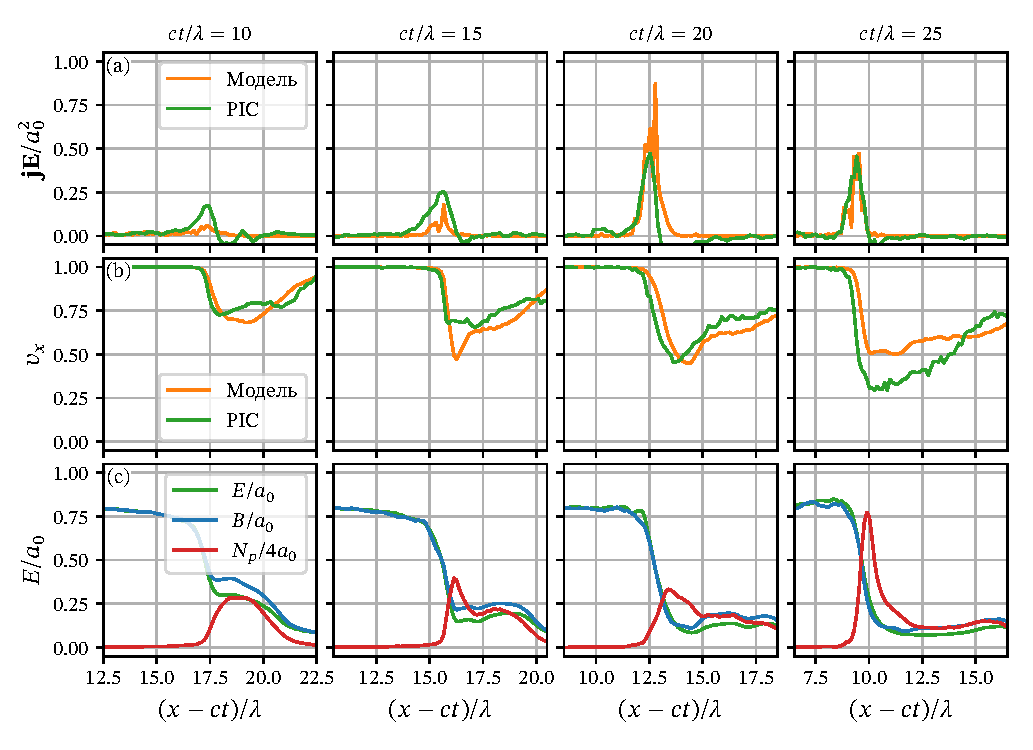
\includegraphics[width=175mm]{cushion-assumptions.pdf}}
    \caption[Проверка приближений аналитической модели развития КЭД каскада в плоской волне]{\label{fig:ch2/sec3/assumptions} 
    Проверка приближений модели. (a), (b) Значение величины $\vb{jE}$ и среднее значение скорости пар $v_x$, рассчитанные по формулам~\eqref{eq:ch2/jE} и~\eqref{eq:ch2/vx} соответственно (оранжевые линии), и взятые напрямую из результатов QED-PIC моделирования (зелёные линии) в различные моменты времени. (c) Распределение амплитуды электрического (зелёные линии) и магнитного (синие линии) полей и концентрации $e^-e^+$ плазмы (красные линии). }
\end{figure}

Предполагая, что время нахождения частицы в вакуумной области достаточно мало, поэтому реакция излучения не успевает существенно влиять на динамику частицы, будем считать, что $\chi\approx\chi_0=\text{const}$.
Тогда
\begin{equation}
    \Delta\varepsilon_\mathrm{rad} = I_\mathrm{rad}(\chi_0)\Delta\varphi.
\end{equation}
Для вычисления величины $\Delta\varphi$ воспользуемся выражениями~\eqref{eq:ch2/sec3/pw_vac_av} и~\eqref{eq:ch2/sec3/deltae_fin}
\begin{equation}
    \mu \varepsilon_\gamma (1 - \cos\theta) = \frac{E^2}{\varepsilon_\gamma (1 - \cos\theta)}\sin^2\frac{\Delta\varphi}{2},
\end{equation}
откуда получаем
\begin{equation}
    \Delta\varphi =  \frac{2\varepsilon_\gamma (1 - \cos\theta)}{E}\sqrt{\mu}
\end{equation}
Учитывая, что $\chi_0 = \chi_\gamma / 2$, выражение для источника $S[\varepsilon_p, \mathrm{rad}]$ записывается в следующем виде
\begin{multline}
    S[\varepsilon, \mathrm{rad}] = \frac{2 \varepsilon_\gamma n_\gamma \sqrt{\mu}}{E} \int_0^\pi \Phi(\theta, v_{\gamma\parallel}) W_\mathrm{pair}(\chi_\gamma, \varepsilon_\gamma) I_\mathrm{rad} \left( \frac{\chi_\gamma}{2} \right)(1 - \cos\theta)\sin\theta d\theta \equiv \\
    \equiv \overline{I_\mathrm{vac}} \frac{\varepsilon_\gamma n_\gamma \sqrt{\mu}}{E} .
\end{multline}

\subsection{Динамика $e^-e^+$ пар в плазменной области}
\label{sub.Pairs}

Согласно рассуждениям в подразделе~\ref{sub:ch2/sec2/Mechanism} в области плотной $e^-e^+$ плазмы в каждой точке пространства существует мгновенная система отсчёта $K'$, движущаяся со скоростью $v_x(x,t)\approx E/B$, в которой присутствует только магнитное поле.
В связи с простотой конфигурации ЭМ поля в $K'$, удобно проводить вычисления в этой системе отсчёта.
В $K'$ электроны и позитроны движутся вдоль магнитного поля со скоростью $v_B'$, а также вращаются в плоскости, перпендикулярной магнитному полю, со скоростью $v_\perp'$ (см. Рис.~\ref{fig:ch2/sec3/plasma}). 
Предположим, что частицы остаются в данной системе отсчёта ультрарелятивистскими (что подтверждается результатами QED-PIC моделирования), тогда справедливо равенство ${v_\perp'}^2+{v_B'}^2\approx1$.
Отметим, что движение заряженных частиц вдоль магнитного поля может приводить к появлению ненулевого тока, который необходимо учитывать в уравнениях Максвелла, тогда как их вращение в магнитном поле в среднем не создаёт ток, однако приводит к генерации гамма-квантов.
Вычислим значение КЭД параметра $\chi$, являющегося Лоренц-инвариантом, в $K'$
\begin{equation}
    \chi_p=\frac{v_\perp'\varepsilon_p'B'}{a_\mathrm{S}} .
\end{equation}
Величины в $K'$ могут быть вычислены по соответствующим величинам в лабораторной системе отсчёта следующим образом: $B'=B\sqrt{1-(E/B)^2}$, $\varepsilon_p'=\varepsilon_p\sqrt{1-(E/B)^2}$, где мы использовали тот факт, что средний импульс частиц вдоль оси $x$ равен $\gamma v_x$ и $v_x=E/B$.
Таким образом значение $\chi$ может быть вычислено следующим образом
\begin{equation}
    \label{eq:ch2/chip}
    \chi_e = \frac{v_\perp'\varepsilon_p E}{a_\mathrm{S}} \frac{1-v_x^2}{v_x} .
\end{equation}
В связи с вращением частиц в магнитном полем, можно предположить, что их угловое распределение в $K'$ близко к изотропному.
В таком случае, аналогично процедуре с гамма-квантами в подразделе~\ref{sub:ch2/sec3/gammas}, функция распределения пар в лабораторной системе отсчёта записывается в следующем виде
\begin{align}
    \label{eq:ch2/distr}
    f_p(t,x,\theta)=\Phi\left(\theta, v_x(x,t)\right) n_p(x,t) .
\end{align}
где $\Phi$ определяется так же, как в уравнении~\eqref{eq:ch2/Phi}
\begin{equation}
    \Phi(\theta,v) = \frac{1-v^2}{{2\left( 1 - v \cos{\theta}  \right)}^2} . \nonumber
\end{equation}
Результаты QED-PIC моделирования, представленные на Рис.~\ref{fig:ch2/sec3/ang} (c), (d) демонстрируют, что выражение~\eqref{eq:ch2/distr} является хорошей аппроксимацией для вычисления углового распределения пар.
Ниже будет показано, что величина $v_x$ может быть приближённо рассчитана из локальных значений электрического поля и концентрации плазмы.
В связи с этим, мы не пишем уравнения переноса величины $v_x$, подобно уравнению~\eqref{eq:ch2/hd_g2}.
Отметим также, что в случае пар мы пренебрегаем разницей между скоростью $v$ системы отсчёта, в которой распределение частиц является изотропным, и средней скоростью частиц $\overline{v}$, вычисленной по такому распределению, т.к. их максимальная разница не превышает $0.2$ согласно выражению~\eqref{eq:ch2/av_vx}.

\begin{figure}
    \centerfloat{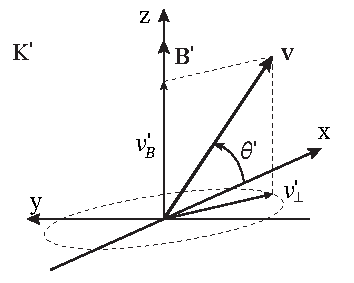
\includegraphics{cushion-plasma.pdf}}
    \caption[Геометрическое расположение скорости и магнитного поля в системе отсчёта $K'$]{\label{fig:ch2/sec3/plasma} Геометрическое расположение скорости и магнитного поля в системе отсчёта $K'$, движущейся со скоростью $v_x=E/B$.}
\end{figure}

Так как величина $\chi_p$ не зависит от угла $\theta$, то источники $S[\alpha, rad_a]$ вычисляются следующим образом
\begin{align}
    S[n, \mathrm{rad_a}] = n_p \int\limits_0^\pi \Phi(\theta, v_x) W_\mathrm{rad}(\chi_p, \varepsilon_p)  \sin\theta d\theta \equiv \overline{W_\mathrm{pl}} n_p, \\
    S[\varepsilon, \mathrm{rad_a}] =  n_p \int\limits_0^\pi \Phi(\theta, v_x) I_\mathrm{rad}(\chi_p)  \sin\theta d\theta \equiv \overline{I_\mathrm{pl}} n_p, \\
    S[v, \mathrm{rad_a}] =  n_p \int\limits_0^\pi \Phi(\theta, v_x) \cos\theta W_\mathrm{rad}(\chi_p, \varepsilon_p)  \sin\theta d\theta  \equiv \overline{W_\mathrm{pl}} v_x n_p.
\end{align}

Суммарная плотность тока частиц, усреднённая по характерному периоду Ларморовского вращения $\tau_B = \varepsilon_p/B$, вычисляется следующим образом
\begin{gather}
    \label{eq:ch2/j}
    \vb{j} = 2 n_p \frac{\vb B}{B} v_B \sqrt{1-v_x^2}, \\
    v_B = v_B' \frac{2}{\pi}\frac{\arccos{(v_x\sqrt{1-v_x^2})}}{\sqrt{1-v_x^2(1-v_x^2)}}\equiv \nu.
\end{gather}
Множитель 2 учитывает тот факт, что токи электронов и позитронов сонаправлены.
Это в свою очередь объясняется из наблюдения, что в лабораторной системе отсчета электрическое и магнитное поля нестрого перпендикулярны.
Таким образом, в системе отсчета $K'$ существует небольшое электрическое поле, направленное вдоль или против магнитного (в зависимости от знака произведения $\vb{E\cdot B}$).
Наличие этого поля приводит к тому, что средняя скорость электронов противонаправлена ему, а средняя скорость позитронов сонаправлена ему.
При этом продольный дрейф частиц не зависит от знака заряда, поэтому токи электронов и позитронов вдоль оси $x$ компенсируют друг друга, а в плоскости $yz$ суммируются.
Этот факт также указывает на то, что электрон-позитронная плазма является проводящей средой, поэтому некоторое поглощение электромагнитной энергии также происходит в этой области, хотя оно и значительно меньше, чем поглощение в вакуумной области, наблюдаемое в QED-PIC моделировании  (см. Рис.~\ref{fig:ch2/sec3/assumptions} (a)) и, таким образом, мы не учитываем его в нашей модели.
Значение $v_B$, усреднённое по частицам, которое мы обозначили как $\nu$, является вторым свободным параметром нашей модели.
Его можно грубо оценить, заметив, что для одиночной частицы значение $v_B'$ может лишь незначительно изменить своё начальное значение в связи с присутствием слабого электрического поля в $K'$.
При этом частицы входят в область плазмы после ускорения лазерным импульсом с преимущественно продольной скоростью, т.е. скоростью вдоль оси $x$, поэтому начальная проекция скорости частиц на магнитное поле, лежащее в плоскости $yz$, является маленькой величиной.
Таким образом, можно ожидать, что наша модель должна давать достоверные результаты при значениях $\nu$, близких к нулю.

Вычисление электродинамических свойства среды, отклик которой на плоскую ЭМ волну состоит в генерации тока вдоль магнитного поля, рассмотрено в следующем разделе. 
Основной вывод состоит в том, что соотношение между электрическим и магнитным полями в такой среде может быть выражено через плотность и амплитуду электрического поля следующим образом
 \begin{equation}
    \label{eq:ch2/vx}
     \frac{E}{B}=v_x=\sqrt{\frac{2}{1+\sqrt{1+\left(4n_p\nu/E \right)^2}}} .
 \end{equation}
Справедливость выражения~\eqref{eq:ch2/vx} также подтверждается путём прямого сравнения с результатами QED-PIC моделирования, продемонстрированного на Рис.~\ref{fig:ch2/sec3/assumptions} (b).


\subsection{Электродинамические свойства $e^-e^+$ плазмы}
\label{app.Electrodynamics}

Рассмотрим распространение плоской циркулярно-поляризованной ЭМ волны вдоль оси $x$ в слабо неоднородной (также вдоль оси $x$) среде, отклик которой на эту волну заключается в генерации тока $\vb{j}=2n_p\vb{v}$, <<опережающего>> электрическое поле волны на половину периода.
Для этого запишем уравнения Максвелла
\begin{align}
    \label{eq:ch2/B.Maxwell1}
    &\pdv{ E_z}{ x} = \pdv{ B_y}{ t}, \\
    \label{eq:ch2/B.Maxwell2}
    &\pdv{ E_y}{ x} = -\pdv{ B_z}{ t}, \\
    \label{eq:ch2/B.Maxwell3}
    &\pdv{ B_z}{ x} = -\pdv{ E_y}{ t} - 2 n_p v_y, \\
    \label{eq:ch2/B.Maxwell4}
    &\pdv{ B_y}{ x} = \pdv{ E_z}{ t} + 2 n_p v_z.
\end{align}
Перейдём к следующим комплексным переменным
\begin{align}
    &\epsilon=E_y+iE_z, 
    \label{eps} \\
    &\beta=B_z-iB_y, \\
    &v_y+iv_z=\frac{\epsilon}{|\epsilon|}iv_{\perp} ,
\end{align}
Введём также вектор-потенциал $a$ следующим образом
\begin{equation}
    \epsilon=-\pdv{ a}{ t} \text{, } \beta=\pdv{ a}{ x}.
\end{equation}
В новых переменных уравнения~\eqref{eq:ch2/B.Maxwell1}--\eqref{eq:ch2/B.Maxwell4} переписываются в следующем виде
\begin{equation}
    \pdv[2]{ a}{ x}=\pdv[2]{ a}{ t}-2 n_p \pdv{ a}{ t}\left| \pdv{ a}{ t} \right|^{-1} iv_\perp.
\end{equation}
Будем искать решение этого уравнения в виде монохроматической плоской волны с амплитудой, зависящей от координаты $x$
\begin{equation}
    a=E(x)e^{i\int^{x}\kappa(x)dx-it},
    \label{a}
\end{equation}
где $E(x)$ и $\kappa(x)$~---~действительные функции координаты $x$, имеющие смысл амплитуды и волнового числа волны.
В итоге уравнения имеют следующий вид
\begin{align}
    \label{eq:ch2/B.Cushion1}
    \pdv[2]{ E}{ x}+E(1-\kappa^2)+2 n_p v_{\perp} =0, \\
    \label{eq:ch2/B.Cushion2}
    E \pdv{ \kappa}{ x} + 2\kappa \pdv{ E}{ x} = 0.
\end{align}
Если плазма является слабо неоднородной, то можно применить приближение ВКБ для решения данного уравнения.
Предполагая, что масштаб неоднородности плазмы $L$ существенно превышает длину волны $\lambda$, можно пренебречь слагаемыми со второй производной: $\partial^2E/\partial x^2 \sim E/L^2 \ll \kappa^2 E = (2\pi)^2E/\lambda^2$.
В таком случае имеем
\begin{equation}
    E(1-\kappa^2)+2 n_p v_{\perp} = 0.
\end{equation}
Решая это уравнение, получаем
\begin{equation}
    \label{eq:ch2/B.kappa}
    \kappa \equiv \frac{B}{E}=\sqrt{1+\frac{2 n_p v_{\perp}}{E}},
\end{equation}
Воспользуемся выражением~\eqref{eq:ch2/j} для $v_\perp$, т.е.
\begin{equation}
v_\perp = \nu \sqrt{1-v_x^2}.
\label{vp}
\end{equation}
Отметим, что в случае $\nu>0$ согласно~\eqref{eq:ch2/B.kappa}, $B>E$, и поэтому $1/\kappa$ имеет смысл дрейфовой скорости $v_x$.
Таким образом,
\begin{equation}
    \frac{1}{v_x}=\sqrt{1+\frac{2n_p\nu}{E}\sqrt{1-v_x^2}} .
\end{equation}
Решение данного уравнения имеет следующий вид
\begin{gather}
    \label{eq:ch2/B.vx}
    v_x= {\left( \frac{2}{1+\sqrt{1+S^2}} \right)}^{1/2},\\
    S=\frac{4n_p\nu}{E}.
\end{gather}
Сравнение полученного решения с численным решением уравнений~\eqref{eq:ch2/B.Cushion1}--\eqref{eq:ch2/B.Cushion2} продемонстрировано на Рис.~\ref{fig.ch2/sec3/ED} как в случае применимости, так и неприменимости приближения ВКБ.
Решение~\eqref{eq:ch2/B.vx} получено в предположении, что $v^2 = 1$, таким образом полученное оно справедливо в системе отсчёта, где частицы являются ультрарелятивистскими, в частности в лабораторной системе отсчёта. 

\begin{figure}
	\centerfloat{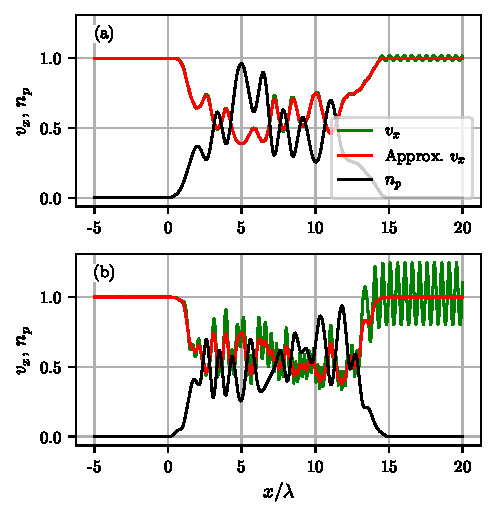
\includegraphics{cushion-ED.pdf}}
	\caption[Дрейфовая скорость частиц в электрон-позитронной плазме]{\label{fig.ch2/sec3/ED} 
    \fixme{Дрейфовая скорость $v_x=E/B$, рассчитанная из численного решения уравнений~\eqref{eq:ch2/B.Cushion1}--\eqref{eq:ch2/B.Cushion2} (зелёная линия) и с помощью аналитического выражения~\eqref{eq:ch2/B.vx} (красная линия) для случайно-неоднородного распределения плазмы (чёрная линия). Масштаб неоднородности превышает длину волны на подрисунке (а), что делает приближение ВКБ справедливым, и меньше её на подрисунке (b).}}
\end{figure}

\subsection{Формулировка модели и сравнение с QED-PIC моделированием}
\label{sub:ch2/sec3/Discussion}

Последние оставшиеся неопределёнными величины~---~это параметры $\psi_\mathrm{vac}$ и $\psi_\mathrm{pl}$, которые разделяют в пространстве вакуумную и плазменную области.
Отметим, что по продольной скорость пар $v_x$, определяемой согласно уравнению~\eqref{eq:ch2/vx}, можно легко различить эти области: в вакууме $v_x\approx 1$, тогда как в плазменной области $v_x < 1$.
Поэтому можно выбрать $\psi_\mathrm{vac}$ и $\psi_\mathrm{pl}$ следующим образом
\begin{align}
    \psi_\mathrm{vac} = v_x^M \\
    \psi_\mathrm{pl} =  1 - v_x^M
\end{align}
где $M\sim 10$~---~достаточно большая константа.
Значение данной константы подбирается исходя из некого условного порога величины $v_x$, при превышении которого можно предположить, что плазма достаточно редкая и и коллективными эффектами можно пренебречь.
Далее будем полагать, что данный порог соответствует величине $0.7$, и $M=8$.

Таким образом, уравнения, описывающие развитие КЭД каскада в плоской волне, имеют следующий окончательный вид
\begin{align}
    \label{eq:ch2/fin1}
    \frac{\partial }{\partial t}n_p  +\frac{\partial}{\partial x}\left( v_x n_p \right) &= \overline{W_\mathrm{pair}} n_\gamma  ,\\
    \label{eq:ch2/fin2}
    \phantom{abs} &= 
    \begin{multlined}[c]
        \mathllap{\frac{\partial}{\partial t}\left( \varepsilon_p n_p \right)  + \frac{\partial}{\partial x}\left( v_p \varepsilon_p n_p \right) \quad}
        \overline{W_\mathrm{pair}} n_\gamma \frac{\varepsilon_\gamma}{2}  + \\
        + n_\gamma\varepsilon_\gamma  \mu \left( \overline{G_\mathrm{rad}} - \frac{\overline{I_\mathrm{vac}}}{\sqrt{\mu} E}  \right) \psi_\mathrm{vac} - \overline{I_\mathrm{pl}} n_p \psi_\mathrm{pl} ,
    \end{multlined} \\
    \label{eq:ch2/fin3}
    \frac{\partial }{\partial t}n_\gamma  +\frac{\partial}{\partial x}\left( \overline{v_{\gamma\parallel}} n_\gamma \right)&=-\overline{W_\mathrm{pair}} n_\gamma + 2\overline{W_\mathrm{rad}} n_p \psi_\mathrm{pl} ,\\
    \label{eq:ch2/fin4}
    \frac{\partial}{\partial t}\left( \overline{v_{\gamma\parallel}} n_\gamma \right) + \frac{\partial}{\partial x}\left( \overline{v_{\gamma\parallel}^2} n_\gamma \right) &= -\overline{V_\mathrm{pair}} n_\gamma + 2 \overline{V_\mathrm{rad}} n_p \psi_\mathrm{pl} ,\\
    \label{eq:ch2/fin5}
    \frac{\partial}{\partial t}\left( \varepsilon_\gamma n_\gamma \right) +\frac{\partial}{\partial x}\left( \overline{v_{\gamma\parallel}} \varepsilon_\gamma n_\gamma \right) &=-\overline{W_\mathrm{pair}}n_\gamma\varepsilon_\gamma   +2 \overline{I_\mathrm{pl}} n_p \psi_\mathrm{pl} ,\\
    \label{eq:ch2/fin6}
    \frac{\partial }{\partial t}\left( \frac{E^2 + E^2/v_x^2}{2} \right) +\frac{\partial}{\partial x} \left( \frac{E^2}{v_x} \right) &=  -2\mu E^{2/3}\varepsilon_\gamma^{1/3}\overline{G_\mathrm{rad}} n_\gamma\psi_\mathrm{vac}  ,\\
    \label{eq:ch2/fin7}
    \frac{\partial }{\partial t}\Sigma_\gamma &=  \overline{I_\mathrm{vac}} n_\gamma \psi_\mathrm{vac} .
\end{align}

Отметим, что в нашей модели сохраняется полная энергия, т.е.
\begin{equation}
    \int \left( 2n_p\varepsilon_p + n_\gamma \varepsilon_\gamma + \frac{E^2 + B^2}{2} \right) dx + \Sigma_\gamma = \text{const} .
\end{equation}


\subsection{Аналитические оценки}
\label{sub:ch2/sec3/analytics}
Перед переходом к численному решению данных уравнений и сравнению в результатами QED-PIC моделирования, сделаем некоторые очень грубые, но аналитические оценки.
\fixme{Мы будем предполагать, что электроны и позитроны излучают гамма-кванты строго против оси $x$.
% Эти гамма-фотоны в свою очередь с вероятностью $W_\mathrm{pair}$ могут распадаться на пары.
Распределение лазерной интенсивности будем считать постоянным и однородным.
В связи с последним предположением, вероятности $W_\mathrm{pair}$ и $W_\mathrm{rad}$ также будем считать постоянными величинами.
В таком случае уравнения непрерывности для концентрации плазмы $n_p$ и фотонов $n_\gamma$ записываются следующим образом в системе отсчёта, движущейся со скоростью $v_x$:}
\begin{align}
	\label{dnpdt}
    \pdv{n_{p}}{ t}  & =    W_\mathrm{pair}n_{\gamma}, \\
	\label{dngdt}   
    \pdv{ n_{\gamma}}{ t}-\pdv{ n_{\gamma}}{ x} &  =   -W_\mathrm{pair}n_{\gamma}+2W_\mathrm{rad}n_{p}
\end{align}
Если пренебречь в \eqref{dngdt} слагаемым с $\partial_x$, характеризующим пространственную дисперсию, то уравнения непрерывности переходят в уравнения, описывающие КЭД каскад во вращающемся электрическом поле без пространственной динамики~\cite{bashmakov2014effect,grismayer2017seeded}.
Уравнения~\eqref{dnpdt}--\eqref{dngdt} можно решить с помощью одностороннего преобразования Фурье \cite{LL10}, т.е. разложения решения на сумму экспонент с действительными значениями $k$ и комплексными значениями $\omega$:
\begin{equation}
    \label{t-x}
    n_{p,\gamma}\left(t,x\right) = \intop_{-\infty+i\sigma}^{+\infty+i\sigma}\mathrm{e}^{-i\omega t}\frac{d\omega}{2\pi}\intop_{-\infty}^{+\infty}\mathrm{e}^{ikx}n_{p,\gamma}\left(\omega,k\right)\frac{\dd k}{2\pi}.
\end{equation}
где
\begin{equation}
    \label{w-k}
n_{p,\gamma}\left(\omega,k\right) = \intop_{0}^{+\infty}\mathrm{e}^{i\omega t}dt\intop_{-\infty}^{+\infty}\mathrm{e}^{-ikx}n_{p,\gamma}\left(t,x\right)\dd x,
\end{equation}
и $\sigma$~---~такое действительное число, что контур интегрирования лежит в области аналитичности $n_{p,\gamma}$. 
Для начальных распределений плотности плазмы и гамма-квантов равных 
$n_{p}\left(0,x\right)$ и $n_{\gamma}\left(0,x\right)$ соответственно, решение находится следующим образом:
\begin{equation}
    \label{np}
    n_{p}\left(t,x\right) = \intop_{-\infty+i\sigma}^{+\infty+i\sigma}\frac{\dd\omega}{2\pi}\intop_{-\infty}^{+\infty}\frac{\dd k}{2\pi}\intop_{-\infty}^{+\infty}dx' 
    \frac{W_\mathrm{pair}n_{p}(0,x')+i\left(\omega+k\right)n_{\gamma}(0,x')}{\Delta\left(\omega,k\right)} \mathrm{e}^{ik(x-x')-i\omega t}
\end{equation}
где $\Delta\left(\omega,k\right)=\omega^{2}+\omega(k + iW_\mathrm{pair})+2W_\mathrm{pair}W_\mathrm{rad}$. 
Возмущения начального распределения распространяются вдоль характеристик, определяемых дисперсионным уравнением $\Delta\left(\omega,k\right)=0$, имеющим следующее решение: 
\begin{equation}
    \label{dispersion}
    \omega=\frac{-k-i W_\mathrm{pair} \pm\sqrt{(k+i W_\mathrm{pair})^{2}-8 W_\mathrm{pair}W_\mathrm{rad}}}{2}. 
\end{equation}
Групповая скорость этих возмущений равна $v_\mathrm{gr}=\partial\mathrm{Re}[\omega]/\partial k$. 
Анализ дисперсионного соотношения показывает, что возмущения с малыми волновыми числами ($k\ll W_\mathrm{pair}$) наиболее неустойчивы и обладают следующим инкрементом неустойчивости:
\begin{equation}
    \Gamma \equiv \mathrm{Im}\left[\omega\right] =\frac{W_\mathrm{pair}}{2} \left(\sqrt{1+\frac{8 W_\mathrm{rad}}{W_\mathrm{pair}}}-1\right),
    \label{gamma}
\end{equation}
что совпадает с инкрементом неустойчивости КЭД каскада во вращающемся электрическом поле~\cite{bashmakov2014effect,grismayer2017seeded}. 
Из~\eqref{dispersion} получим дисперсионное соотношение для неустойчивых возмущений:
\begin{align}
    \omega & \approx  \frac{\mu-1}{2}k + i\Gamma \\
    \mu & =  \frac{1}{\sqrt{1+8 W_\mathrm{rad}/W_\mathrm{pair}}}.
    \label{omega}
\end{align} 
В пределе $a_0 \rightarrow \infty$, $W_\mathrm{rad}/W_\mathrm{pair} \approx 4$ и $\mu \approx0.17$ \cite{berestetskii1982quantum}. 
Поэтому возмущения с малыми волновыми числами распространяются со скоростью ${v_\mathrm{gr}\approx -0.41}$.
Это значение совпадает с результатами численного решения уравнений~\eqref{dnpdt}--\eqref{dngdt} с различными формами начальных распределений пар и гамма-квантов (см. пример такого решения на Рис.~\ref{front}).

\begin{figure}[h!]
	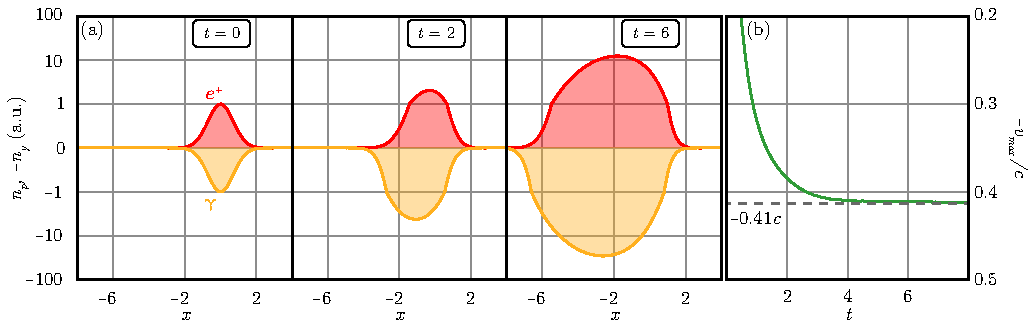
\includegraphics[width=165mm]{front.pdf}
    \caption{\label{front} \fixme{Численное решение уравнений (\ref{dnpdt})--(\ref{dngdt}): (a) Распределение плотности позитронов $n_p$ (красная линия) и гамма-квантов $n_\gamma$ (оранжевая линия) в различные моменты времени. Масштаб вертикальной оси линейный для значений $[-1,1]$ и логарифмический для остальных значений. Координаты, время и плотности нормированы таким образом, что $W_\mathrm{rad}=1.0$, $W_\mathrm{pair}=0.25$.
    (b) Скорость фронта распределения плотности $n_p$, определяемая по порогу $n_p = 0.1$, как функция времени.}}
\end{figure}

В системе отсчёта, движущейся со средней продольной скоростью плазмы, скорость фронта каскада $v_\mathrm{fr}$ совпадает с найденной групповой скоростью $v_\mathrm{gr} \approx -0.41$.
Переход в лабораторную систему отсчёта позволяет связать среднюю продольную скорость частиц плазмы и скорость фронта каскада:
\begin{equation}
    v_\mathrm{fr}=\frac{v_\mathrm{pl}+v_\mathrm{gr}}{1+ v_\mathrm{pl} v_\mathrm{gr} /c^2} 
\label{vcf}
\end{equation}
Решая это уравнение относительно $v_\mathrm{pl}$ получаем:
\begin{equation}
    \label{vpl}
    v_\mathrm{pl}=\frac{v_\mathrm{fr}-v_\mathrm{gr}}{1-v_\mathrm{gr}v_\mathrm{fr}/c^2} 
\end{equation}
Эти рассуждения предсказывают $v_\mathrm{pl}=0.61$ для $v_\mathrm{fr} = 0.27$ ($a_{0}=2500$, см. Рис.~\ref{fig:ch2/cushion-x-t}), что достаточно близко к усреднённой скорости позитронов $\approx 0.75$, полученной из численного моделирования (см. Рис.~\ref{fig:ch2/field-structure}(b)).

\subsection{Численное решение}
\label{sub:ch2/sec3/Numeric}

Численное решение уравнений~\eqref{eq:ch2/fin1}--\eqref{eq:ch2/fin6} находится по методу линий: частные производные $\partial/\partial x$ аппроксимируются конечными разностями для получения системы ОДУ, которая решается с помощью явного метода Рунге-Кутты.
Так как метод Рунге-Кутты не является симплектическим, то сохранение энергии на каждом шаге интегрирования соблюдается путем отсечения производной $\partial n_\gamma /\partial t$ так, чтобы полная энергия не росла.
Относительная ошибка, полученная в результате этой процедуры, оказывается приемлемо малой.
Свободные параметры оценивались вручную путем сравнения решения с результатами трехмерного QED-PIC моделирования на основе двух макроскопических параметров: скорости фронта каскада и энергетического баланса в системе.
После тестирования редуцированной модели выяснилось, что существует положительная корреляция между параметром $\nu$ и скоростью распространения фронта каскада.
Параметр $\mu$ в основном определяет передачу энергии от лазера к каскадным частицам, поэтому, изменяя этот параметр, можно управлять характерным временем исчерпания энергии лазера.
Отметим, что расчетные значения параметров подгонки практически равны друг другу для различных начальных условий (см. рис.~\ref{fig:ch2/sec3/sol2500}--\ref{fig:ch2/sec3/sol1000}).

Трехмерное QED-PIC моделирование было выполнено с использованием кода QUILL~\cite{QUILL}, который позволяет моделировать КЭД эффекты с помощью метода Монте-Карло.
Начальное распределение ЭМ полей имеет вид плоской волны с длиной волны $\lambda=2\pi c/\omega_{L}=\SI{1}{\um}$ и амплитудой $a_0 $, распространяющееся вдоль оси $x$ с пространственно-временной огибающей, задаваемой следующим выражением
\begin{equation}
a(x,y,z) =  \cos^2 \left( \frac{ \pi }{2}   \frac{x^4}{\sigma_x^4 } \right) \cos^2 \left( \frac{ \pi}{2}   \frac{\left( y^2 + z^2 \right)^2}{\sigma_r^4 } \right)
\end{equation}
Поперечный пространственный размер лазерного импульса составлял $2\sigma_r = \SI{18}{\um}$, а длительность импульса $\SI{60.5}{\femto\second}$ ($2\sigma_x = \SI{18.15}{\um}$).
Размер области модулирования составлял $30\lambda\times 30\lambda\times 30\lambda$, количество ячеек $3000\times 300\times 300$.
Как обсуждалось в подразделе~\ref{sub:ch2/sec2/Mechanism}, финальная стадия развития каскада КЭД в одиночном лазерном импульсе практически не зависит от затравки, поэтому мы выбираем затравку в виде короткого гамма-сгустка, распространяющегося навстречу лазерного импульса, чтобы не учитывать взаимодействие с электрон-ионной плазмой, существенно отличающейся от формирующейся электрон-позитронной плазмы.
Начальная затравка в таком виде в нашей модели может быть задана путём инициализации $v_{\gamma\parallel}(t=0)\approx-1$.
Распределения плотности в нашей модели и PIC-моделировании совпадают и выражаются следующей формулой: $n_\gamma(t=0)=n_0\max\left\{0, 1 - (x-x_0)^2/w_\gamma ^2 \right\}$, где $w_\gamma$~---~полуширина сгустка, а $x_0$~---~положение его центра.
Начальная энергия гамма-квантов была установлена равной $200 m_e c^2$.

\begin{figure}
    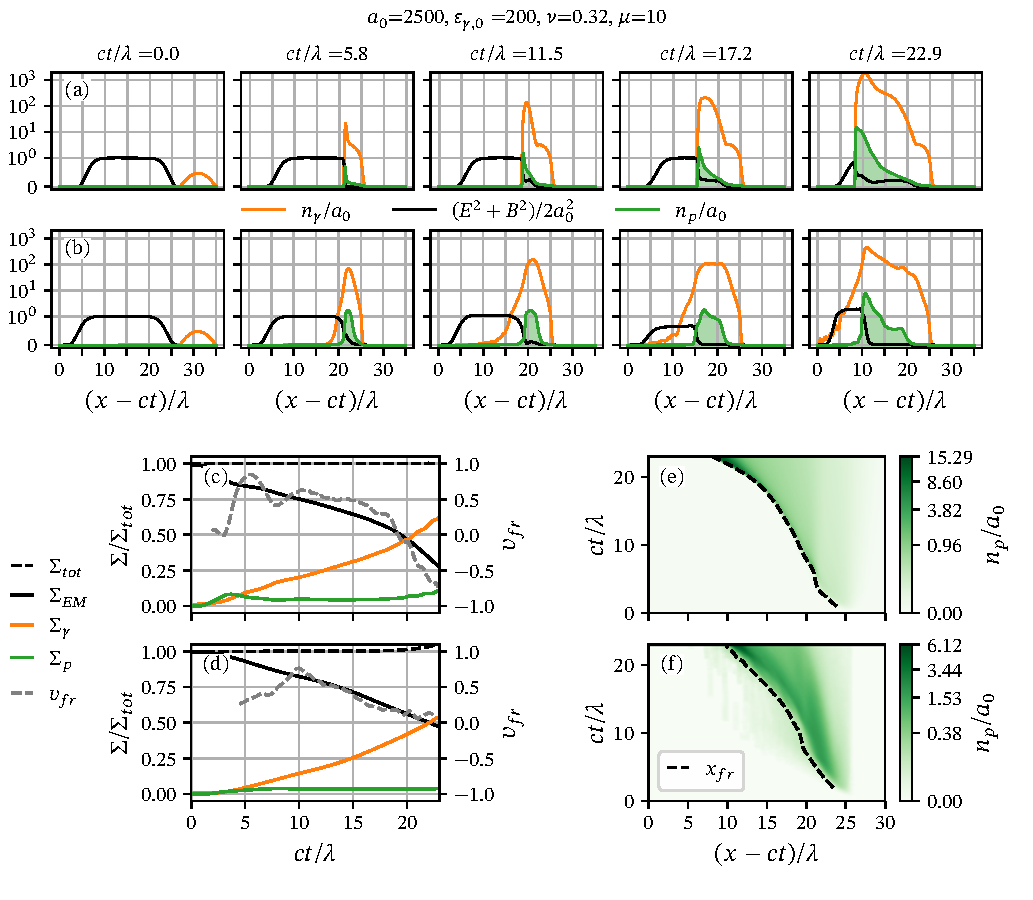
\includegraphics{cushion-sol-2500-new.pdf}
    \caption[Сравнение решения модельных уравнений, описывающий развитие КЭД каскада и результатов QED-PIC моделирования для начальных параметров $a_0=2500$, $n_{\gamma,0}=0.5 a_0 n_\mathrm{cr}$]{\label{fig:ch2/sec3/sol2500} 
    Сравнение между (a, c, e) решением уравнений~\eqref{eq:ch2/fin1}--\eqref{eq:ch2/fin6} и (b, d, f) результатами QED-PIC моделирования для начальных параметров $a_0=2500$, $n_{\gamma,0}=0.5 a_0 n_\mathrm{cr}$.
    (a, b) Распределение концентрации гамма-квантов $n_\gamma$, плотности ЭМ энергии $(E^2+B^2)/2$ и концентрации плотности плазмы $n_p$ в различные моменты времени.
    Вертикальная шкала является линейной в диапазоне $[0,\ 1]$ и логарифмической в диапазоне $[1,\ +\!\infty]$.
    (c, d) Баланс энергии в системе: полная энергия $e^-e^+$ пар $\Sigma_p$, гамма-квантов $\Sigma_\gamma$ и ЭМ энергия $\Sigma_{EM}$, нормированные на полную начальную энергию системы $\Sigma_{tot}$; скорость фронта каскада $v_\mathrm{fr}$.
    (e, f) Распределение $e^-e^+$ пар в плоскости $x$, $t$ и положение фронта каскада $x_\mathrm{fr}$. Значения свободных параметров модели: $\nu=0.32$, $\mu=10$.}
\end{figure}

Прямое сравнение между решениями уравнений ~\eqref{eq:ch2/fin1}~--~\eqref{eq:ch2/fin6} и результатами QED-PIC моделирования показано на Рис.~\ref{fig:ch2/sec3/sol2500}~--~\ref{fig:ch2/sec3/sol1000}.
Наша модель качественно совпадает с результатами QED-PIC моделирования с точки зрения распределения частиц и электромагнитного поля, а также энергетического баланса.
Также отчетливо различаются режимы развития каскада как в нашей модели, так и в QED-PIC моделировании.

Первый режим реализуется, когда значение $a_0$ лазерного импульса недостаточно велико или гамма-сгусток недостаточно плотный.
В этом случае плотность образующейся электрон-позитронной плазмы не достигает релятивистской критической плотности, так что $v_x\approx 1$, т.е. не возникают коллективные плазменные эффекты.
В этом случае плазменная область вообще отсутствует, а вновь рождающиеся частицы движутся в неизменном поле лазерного импульса, близком к плоской волне.
Как обсуждалось в работах~\cite{di2012extremely, bulanov2013electromagnetic, narozhny2015quantum, mironov2017observable} (\fixme{в главе 1}), в этом случае значение параметра $\chi$ пар не растет при движении в плоской волне.
Но после каждого акта испускания гамма-кванта величина $\chi$ делится между родительской и дочерней частицами, так что через несколько поколений $\chi$ всех частиц становится пренебрежимо малым и развитие каскада прекращается.
Таким образом, при достаточно малых $a_0$ гамма-кванты гамма-сгустка распадаются на пары, оставляющие <<шлейф>> электронов и позитронов, которые ускоряются вперед и распространяются вместе с лазерным импульсом.
Хотя плотность плазмы мала, общее количество пар может быть достаточно большим, чтобы значительная часть лазерной энергии передавалась им (см. Рис.~\ref{fig:ch2/sec3/sol1000} (c), (d) ).
Поскольку в этом режиме все частицы распространяются независимо друг от друга, фронт каскада распространяется с почти постоянной скоростью $v_\mathrm{fr}\approx -0.5$.

\begin{figure}[ht]
    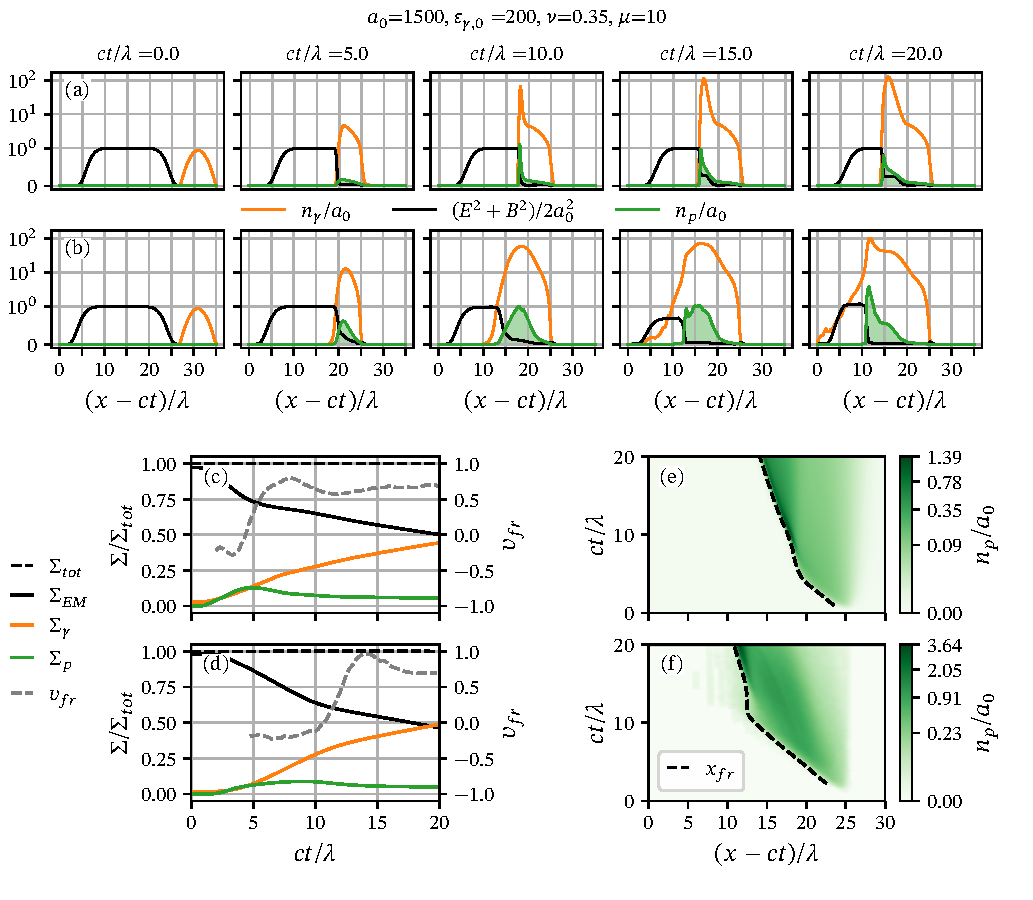
\includegraphics{cushion-sol-1500-new.pdf}
    \caption[То же, что на Рис.~\ref{fig:ch2/sec3/sol2500} для начальных параметров $a_0=1500$, $n_{\gamma,0}=a_0 n_\mathrm{cr}$]{\label{fig:ch2/sec3/sol1500} 
    То же, что на Рис.~\ref{fig:ch2/sec3/sol2500} для начальных параметров $a_0=1500$, $n_{\gamma,0}=a_0 n_\mathrm{cr}$. Значения свободных параметров модели: $\nu=0.35$, $\mu=10$.}
\end{figure}

% The first regime is observed when $a_0$ of the laser pulse is not big enough or the gamma-bunch is not dense enough. In that case the density of the produced electron-positron plasma does not reach the relativistic critical density so that $v_x\approx 1$, i.e. the collective plasma effects do not occur. In this case the plasma region is not present at all and the newly born particles move in the unaltered field of the laser pulse which is close to the plane wave. As discussed in~\cite{DiPiazza2012, bulanov2013electromagnetic, narozhny2015quantum, mironov2017observable} in that case $\chi$ of the pairs does not grow during its motion in the plane wave. But after each act of the gamma-quant emission it splits between the parent and the child particles so after few generations $\chi$ of all the particles becomes negligibly small so the cascading ceases. Thus for small enough $a_0$ the gamma-quanta of the gamma-bunch decay into pairs levaing the `trail' of the electrons and positrons which are accelerated forwards and co-propagate with the laser pulse. Although the density of the plasma is small the total number of the pairs can be big enough so that the significant portion of the laser energy is transferred to them [see Fig.~\ref{fig:ch2/sec3/sol1000} (c), (d)]. Because in this regime all the particles propagate independently to each other the cascade front propagates with almost constant velocity $v_\mathrm{fr}\approx -0.5$.

Во втором режиме каскад развивается, как обсуждалось в подразделе~\ref{sub:ch2/sec2/Mechanism}.
Пик плотности пар распространяется в сторону лазера со значительно меньшей скоростью (относительно переднего фронта лазерного импульса), чем в первом режиме.
При этом плотность плазмы растет во времени в отличие от первого режима, когда плотность плазмы в каждой точке остается практически неизменной после прохождения этой точки начальным гамма-сгустком.
Как упоминалось в п.~\ref{sub.Pairs}, плотная электрон-позитронная плазма фактически почти не поглощает лазерное поле, поэтому, несмотря на то, что в этом режиме общее число пар значительно больше, чем в первом скорости передачи энергии от ЭМ поля к парам близки друг к другу в обоих режимах.

% In the second regime the cascade develops as discussed in Sec.~\ref{sec.Introduction}. The peak of the pairs density propagates towards the laser with a much slower velocity (relative to the leading edge of the laser pulse) than in the first regime. Moreover the density of the plasma grows in time in contrast to the first regime where the plasma density at each point stays almost the same after the initial gamma-bunch passes that point. As mentioned in Sec.~\ref{sub.Pairs} the dense electron-positron plasma actually almost does not absorb the laser field that is why despite the fact that in this regime the total number of the pairs is much larger than in the first regime, the rates of the energy transfer from the EM field to the pairs are close to each other in both regimes.

\begin{figure}[ht]
    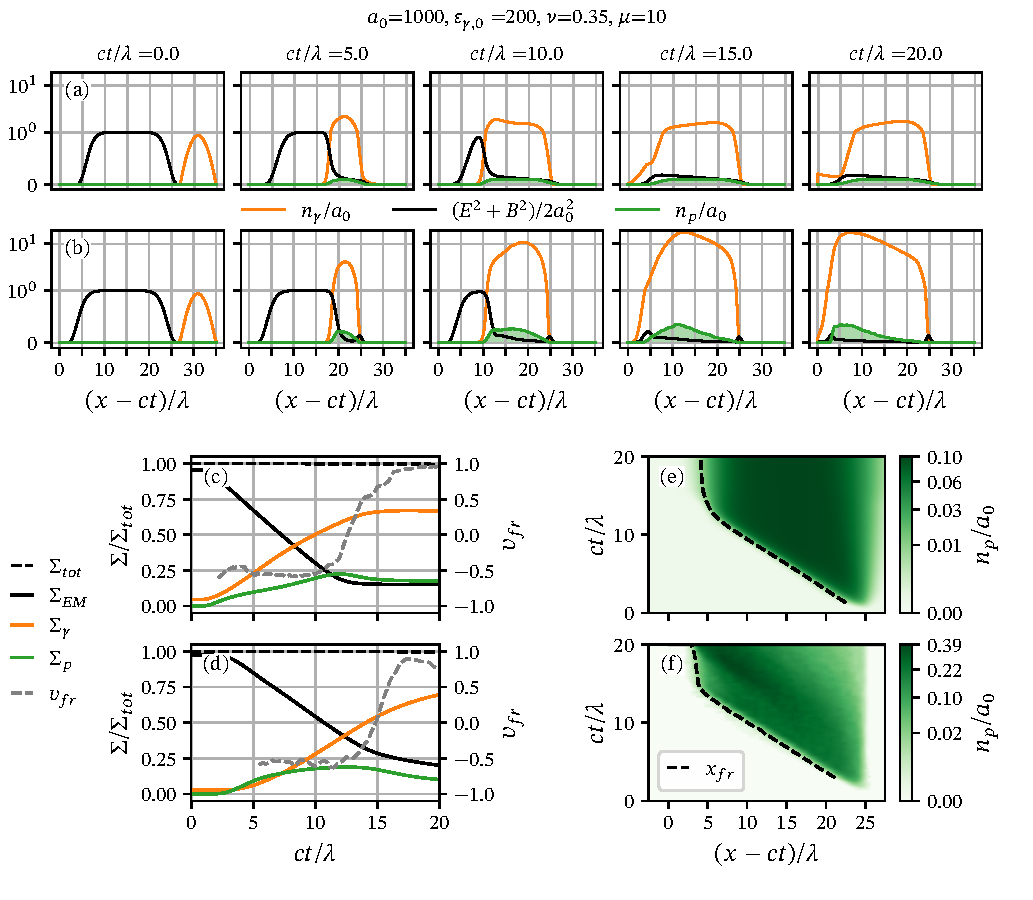
\includegraphics{cushion-sol-1000-new.pdf}
    \caption[То же, что на Рис.~\ref{fig:ch2/sec3/sol2500} для начальных параметров $a_0=1000$, $n_{\gamma,0}=a_0 n_\mathrm{cr}$]{\label{fig:ch2/sec3/sol1000} 
    То же, что на Рис.~\ref{fig:ch2/sec3/sol2500} для начальных параметров $a_0=1000$, $n_{\gamma,0}=a_0 n_\mathrm{cr}$. Значения свободных параметров модели: $\nu=0.35$, $\mu=10$.}
\end{figure}

Если $a_0$ лежит между значениями, при которых наблюдается либо первый, либо второй режим, то на начальном этапе каскад напоминает каскад S-типа, на что явно указывает отрицательное значение скорости фронта каскада (см. синюю пунктирную линию на Рис.~\ref{fig:ch2/sec3/sol1500} (c), (d)). 
В какой-то момент плотность пар становится достаточно большой, чтобы изменить распространение лазера и каскад переходит в режим самоподдержания.
На смену этих двух режимов указывает резкое изменение скорости фронта каскада.
Начальная стадия (стадия каскада S-типа) просматривается и при больших значениях $a_0$ (см. рис.~\ref{fig:ch2/sec3/sol2500}), однако она значительно короче и слабо выражена в результатах QED-PIC моделирования.

% If the $a_0$ lays in-between the values of $a_0$ at which either the first or the second regime is observed, at the initial stage the cascade resembles the S-type cascade which is clearly indicated by the negative value of the velocity of the cascade front [see grey dashed line in Fig.~\ref{fig:ch2/sec3/sol1500} (c), (d)]. At some point the density of the pairs becomes large enough to alter the laser propagation and to shift the cascade dynamics to the self-sustained regime. The change between these two regimes is indicated by abrupt change in the velocity of the cascade front. The initial stage (stage of the S-type cascade) can also be seen for larger values of $a_0$ (see Fig.~\ref{fig:ch2/sec3/sol2500}), though it is much shorter and is hardly pronounced in the results of the QED-PIC simulations.

\fixme{Мы также проверили разработанную выше грубую аналитическую оценку, из которой была получена связь между средней продольной скоростью частиц каскада и скоростью фронта каскада.}
Это предсказание модели, рассчитанное на основе средней скорости частиц каскада, примерно совпадает с реальной скоростью, наблюдаемой в модельном решении (см. Рис.~\ref{fig.former}) на стадии самоподдержания каскада.
Поскольку этот этап никогда не начинается при $a_0 = 1000$, эта упрощенная модель не может быть применена в этом случае.

% We also verified the results of the simplified model developed by us in Ref.~\cite{Samsonov2019} from which a relation between the mean longitudinal velocity of the cascade particles and the cascade front velocity was obtained. This model prediction calculated based on the mean velocity of the cascade particles roughly coinsides with the actual velocity observed in the model solution (see Fig.~\ref{fig.former}) at the stage of the cascade self sustenance. As this stage never starts for $a_0 = 1000$, this simplified model cannot be applied in that case.

Стоит отметить некоторые особенности развития КЭД каскада не воспроизводятся в нашей модели.
Например, в PIC моделировании отчетливо виден <<хвост>> пространственного распределения гамма-квантов, распространяющийся навстречу лазерному импульсу.
Эти гамма-кванты имеют относительно низкую энергию и, следовательно, не могут фотообразовать электрон-позитронные пары.
Наша модель предсказывает, что края распределения плазмы и гамма-квантов почти полностью совпадают.
Суммарная энергия, уносимая такими гамма-квантами, незначительна, поэтому для развития каскада эта особенность не является решающей.
Причина, по которой наша модель не может отразить эту особенность, заключается в том, что мы предполагаем, что функции распределения являются моноэнергетическими.
Более высокую точность можно получить, если разбить гамма-кванты на несколько групп с разными энергиями и описать их отдельно; тогда эта особенность присутствовала бы в наших решениях.
Но, как уже упоминалось в п.~\ref{sub:ch2/sec3/Assumptions}, это сильно усложнит модель, но не приведет к существенным качественным изменениям решений.
% \fixme{Во-вторых, как общее количество пар, так и пиковая плотность плазмы в QED-PIC моделировании больше, чем в нашем модельном решении для меньших значений $a_0$.
% Одной из причин этих расхождений является то, что наша модель является одномерной и, следовательно, не описывает дифракцию лазерного импульса.
% В моделировании 3D-PIC область моделирования всегда ограничена, поэтому при моделировании нельзя получить чистую плоскую волну.}
% Это приводит к тому, что огибающая лазерного импульса эволюционирует так, что величина лазерного импульса в области вакуума может отличаться от его начального значения $a_0$ [см. рис.~\ref{fig:ch2/sec3/assupps} (c )].
% Увеличение эффективной интенсивности лазерного импульса, как правило, приводит к увеличению вероятности процессов КЭД и, следовательно, к более обильному фоторождению пар.
% Суммарный эффект непостоянства интенсивности лазерного импульса можно частично учесть, выбрав значение $a_0$ в модельном решении больше, чем значение, изначально заданное при PIC моделировании.

% There are some features that are not captured by our model which are worth noting. Firstly, in the PIC simulation there is a distinct tail of the gamma-quanta spatial distribution counter-propagating to the laser pulse. These gamma-quanta have relatively low energy and thus are unable to photoproduce pairs. Our model predicts that the edge of the plasma and gamma-quanta distributions almost competely coincide. The total energy carried away by this sort of gamma-quanta is insignificant so this feature is not crucial for the cascade development. The reason that our model cannot capture this feature is the fact that we assume the distribution functions to be monoenergetic. Higher accuracy can be obtained if we would split the gamma-quanta into several groups with different energies and describe them separately; then this feature would be present in our solutions. But as already mentioned in Sec.~\ref{sec.Main} it will greatly complicate the model but will not lead to significant qualitative changes in the solutions.
% Secondly, both the total number of the pairs and peak plasma density are larger in the QED-PIC simulation than in our model solution for smaller values of $a_0$. One of the reasons behind these discrepancies is that our model is 1-dimensional and thus does not describe the laser pulse diffraction. In the 3D-PIC simulations the simulation box is always limited thus the pure plane wave cannot be achieved in the simulations. It leads to the fact that the envelope of the laser pulse evolves so that the magnitude of laser pulse in the vacuum region may differ from its initial value $a_0$ [see Fig~\ref{fig:ch2/sec3/assumptions} (c)]. The increase of the effective laser pulse intensity generally leads to the increase of the probabilities of the QED processes and thus more abundant pairs photoproduction. The net effect of the inconstancy of the laser pulse intensity can be partially accounted by choosing the value of $a_0$ in the model solution larger than the value initially set in the PIC simulation.

% \begin{figure}
%     \includegraphics[width=85mm]{former_model.pdf}
%     \caption{\label{fig.former} Velocity of the cascade front observed in the model solution (green line) and obtained from the simplified model developed in Ref.~\cite{Samsonov2019} (red line) calculated from the mean velocity of the particles located at the $2 \lambda$ depth behind the cascade front.}
% \end{figure}

\section{Выводы}
\label{sec.Conclusion}

Таким образом, мы показали, что самоподдерживающийся КЭД каскад может развиваться в плоской волне, вопреки достаточно распространённому мнению, что такая конфигурация поля является неподходящей для наблюдения КЭД каскадов~\cite{narozhny2015quantum,mironov2017observable,bulanov2013electromagnetic}.
Однако, для наблюдения такого эффекта требуется достаточно плотная затравка, способная влиять на распространение этой плоской волны.
Важно отметить, что при этом наличие отражения падающей волны не является принципиальным, поэтому КЭД каскад в одиночной плоской волне принципиально отличается от такового, например, в стоячей волне, который достаточно активно исследуется в силу наличия аналитических оценок и достаточно низкого порога наблюдения.

Развитие КЭД каскада приводит к эффективному преобразованию падающих оптических фотонов в жёсткие фотоны и электронно-позитронные пары, при этом начальная затравка движется почти со скоростью света.
Таким образом, образуется электрон-позитронная <<подушка>>, фронт которой (граница вакуум-плазма) движется медленнее затравки из-за непрерывного образования электрон-позитронной плазмы.
Подобно волнам ионизации в физике газового разряда~\cite{bollen1983high,semenov1982breakdown}, распространение фронта КЭД каскада можно рассматривать как ударную волну <<пробоя вакуума>>.
Плотность плазмы подушки в конце концов превышает релятивистскую критическую плотность, и плазма экранирует затравочные частицы от падающей волны.
Инкремент роста числа частиц при развитии каскада в поле двух встречных электромагнитных волн с круговой поляризацией рассчитан численно в публикации~\cite{grismayer2017seeded} как функция $a_0$.
Пороговое значение $a_0$ можно оценить из условия удвоения числа частиц в течение лазерного периода.
Для длины волны $\SI{1}{\um}$ пороговое значение $a_0$ составляет около $10^3$.
Из наших расчетов следует, что в плоской волне, порог развития КЭД каскада соответствует примерно величине $a_0 \sim 1500$, что несколько выше порога развития каскада в стоячей волне, но всё ещё значительно ниже критического поля Заутера-Швингера $a_0 \simeq m c^2/ \hbar \omega_\mathrm{L} \simeq 4 \times 10^5 $~\cite{Sauter31, Schwinger51}.
Из наших расчетов следует, что пороговая интенсивность падающей волны составляет около $6 \times 10^{24}$~Вт/см$^2$ для длины волны $\SI{1}{\um}$.
Как указывалось выше пороговая интенсивность для вакуумного пробоя может быть достигнута с помощью будущих лазерных установок, хотя и за счёт использования достаточно острой фокусировки излучения.
Тем не менее выводы данной работы могут быть важны для их приложений.
Возникновение волны пробоя вакуума и последующее поглощение лазерного излучения расширяют ограничения достижимой лазерной интенсивности~\cite{Bell2008, fedotov2010limitations} на случай слабой фокусировки.
Интересной особенностью такого каскада является то, что скорость его фронта, или, другими словами, скорость границы раздела вакуум-плазма, может быть значительно меньше скорости света и почти не зависит от времени.
При этом величина этой скорости фронта уменьшается с увеличением амплитуды падающей волны.
Полученные результаты аналогичны для затравки в виде слоя как электрон-ионной так и электрон-позитронной плазмы.
Независимость (до определённой степени) процесса развития КЭД каскада от затравки также указывает на реализацию самоподдерживающегося режима.

Также нами была разработана аналитическая самосогласованная модель развития такого КЭД каскада.
Полное описание этого взаимодействия требует решения уравнений Максвелла вместе с кинетическими уравнениями для электронов, позитронов и гамма-фотонов.
Эта система уравнений слишком сложна для аналитических методов и обычно решается численно с помощью, например, QED-PIC кодов, требующих много вычислительных ресурсов.
Чтобы получить редуцированные уравнения для вычислительно легкой модели, был сделан ряд предположений, основные из которых заключаются в переходе к квазиодномерному гидродинамическому описанию; использованию локально-квазимоноэнергетических функций распределения частиц и приближения плоской волны для лазерного излучения.
Полученная упрощенная система уравнений записывается в замкнутом виде и решается численно.
Несмотря на сложность и нелинейность динамики каскада, оказалось, что относительно простая одномерная модель позволяет качественно предсказать его развитие, например, макроскопическое пространственно-временное распределение частиц и энергетический баланс в системе.
Этот факт служит обоснованием аналитического обоснования модели и, следовательно, нашего понимания процесса.
% Хотя есть несколько расхождений между предсказаниями нашей модели и результатами QED-PIC моделирования, нами определены причины, лежащие в их основе, и для некоторых предложены методы их устранения.
Методы, используемые для разработки данной модели, вероятно могут быть применены для построения схожих моделей, описывающих астрофизические явления, такие как развитие КЭД каскадов в магнитосферах нейтронных звезд, также отличающихся сложной пространственно-временной динамикой и сопровождающихся генерацией волн пробоя вакуума~\cite{timokhin2010time}.

Основные полученные в данной главе результаты опубликованы в работах~\cite{samsonov2019laser, samsonov2021hydrodynamical, samsonov2021effect, samsonov2018NW, samsonov2019FNP, samsonov2020NW, samsonov2020UFL, samsonov2021UFL}

\FloatBarrier
